\chapter{روش پیشنهادی}

\newpage
‎\renewcommand{\baselinestretch}{2}\normalsize‎
\label{ProposedApproach}

در این فصل روش پیشنهادی برای یادگیری توزیع‌شده در شبکه‌های تطبیقی ناهمگن با هدف کاهش ارتباطات در زمان اجرا و کاهش زمان انتظار گره‌ها و مقابله با مساله کندکننده‌ها ارائه خواهد شد. در ابتدا مقدمات و کلیات روش شرح داده شده و در ادامه جزئیات هر قسمت و تحلیل همگرایی و پایداری روش پیشنهادی بحث خواهد گردید.
\section{روش پیشنهادی}
همان گونه که در بخش تعریف مسئله مطرح شد، هدف از این پژوهش بدین صورت است که با استفاده از مفاهیم موازی‌سازی یک رویکرد یادگیری توزیع‌شده برای تخمین پارامترهای مسائل بهینه‌سازی در شبکه‌های تطبیقی توزیع‌شده ارائه داد. این رویکرد یادگیری توزیع‌شده مبتنی بر یک مدل محاسباتی موازی توسعه‌یافته به نام \lr{BSP} فدرالی (\lr{FBSP}) است که با توجه به خصوصیات شبکه‌های تطبیقی توزیع‌شده توسعه‌ یافته است. 

رویکردهای یادگیری توزیع‌شده به سه دسته همگام، غیرهمگام متمرکز و غیرهمگام غیرمتمركز تقسيم مي‌شوند. الگوریتم‌های همگام در یک محیط ناهمگن عملکرد ضعیفی دارند و الگوریتم‌های غیرهمگام متمرکز از مشکل گلوگاه ارتباطی در سرورهای پارامتر با افزایش تعداد گره‌ها و كاهش ميزان همگرايي با متراكم شدن ترافيك سرور پارامتر  رنج می‌برند. در این رساله به دنبال ارائه یک رویکرد موازی برای شبکه‌های تطبیقی توزیع‌شده هستیم که در عین کارآمد بودن ارتباطات و حفظ بهترین میزان همگرایی، در یک محیط ناهمگن نیز مقاوم باشد. در يك محيط ناهمگن سرعت محاسبه و ارتباطات گره‌های شبکه متفاوت خواهد بود. این امر به ویژگی‌های معماری، اشتراک منابع (به عنوان مثال، محاسبات ابری) و بد عمل كردن سخت افزار وابسته است. از آنجایی‌که هدف این نوع شبکه‌ها تخمین بردار پارامترهای بهینه از طریق تعامل و همکاری بین گره‌های مختلف بدون حضور یک سرور مرکزی است و همچنین به دلیل عدم نیاز انتظار هر گره برای سایر گره‌های شبکه و همچنین عدم نیاز به قفل‌گذاری‌های هزینه‌بر، الگوریتم‌های موازی‌سازی غیرهمگام غیرمتمرکز انتخاب مناسبی برای این شبکه‌ها می‌باشند. 

رویکرد پیشنهادی یک رویکرد داده-موازی است که هر گره بر روی داده‌های محلی خودش فرآیند یادگیری را انجام خواهد داد و در دو مرحله اصلی برون‌خط و برخط اجرا می‌شود. مرحله برون‌خط که مرحله پیش‌پردازش نیز نامیده می‌شود، شامل دو بخش رصدکردن شبکه و منطقه‌بندی شبکه است. در بخش رصد کردن شبکه، توان پردازشی هر گره محاسبه می‌شود. در بخش منطقه‌بندی شبکه، خوشه‌بندی گره‌ها براساس فاصله گره‌ها از همدیگر، توان پردازشی و میزان اعتماد بین گره‌ها انجام می‌شود. در مرحله برخط، فرآیند یادگیری موازی تحت مدل محاسباتی \lr{BSP} فدرالی بر روی شبکه تطبیقی توزیع‌شده که در مرحله پیش‌پردازش منطقه‌بندی شده است، اجرا خواهد شد. 

این مدل همانند مدل \lr{BSP} از سه بخش اصلی محاسبه، ارتباط و همگام‌سازی مانعی تشکیل شده است. با این تفاوت که مرحله ارتباط و همگام‌سازی مانعی در مدل \lr{BSP} فدرالی بر اساس یک روش منطقه‌بندی‌ انجام می‌شود. برای همگام‌سازی گره‌های شبکه در این رویکرد یک تکنیک همگام‌ فدرالی معرفی شده است که گره‌ها به صورت منطقه‌بندی شده و با قبول یک میزان کهنگی در سطح کل گره‌های شبکه همگام می‌شوند. به عبارت دیگر، همگام‌سازی در دو سطح منطقه‌ای و سراسری اجرا خواهد شد. در سطح منطقه‌ای، گره‌های همسایه‌ای با هم همگام می‌شوند که از لحاظ توان محاسباتی بهم شبیه‌ و از لحاظ فاصله ساختاری و میزان اعتماد بهم نزدیک باشند. در سطح سراسری، هر گره با گره‌های همسایه‌اش در کل شبکه همگام می‌شود. این روش منطقه‌بندی سبب می‌شود هزینه ارتباطات بین گره‌ها در زمان اجرا کاهش یابد و از رخ دادن مشکل کندکننده‌ها جلوگیری شود. در ادامه، بخش‌های مختلف راه‌کار پیشنهادی با جزئیات کامل شرح داده شده است.

\section{متغیرهای استفاده شده}
مجموعه متغیرهای استفاده شده در این رساله در جدول \ref{notation} آورده شده است.
\begin{table}[h]	
	\centering
	\caption{\small{متغیرهای مورد استفاده در مدل ریاضی سیستم پیشنهادی}}
	\label{notation}
	\footnotesize\rm
	\begin{tabular}{cc}
		\hline
		متغیر&توصیف\\
		\hline
		$N$&تعداد گره‌ها در شبکه\\
		$M$&مرتبه فیلتر یا اندازه بردار پارامترها\\
		$w_{k,t}$&بردار پارامترها گره \lr{k} در تکرار \lr{t}\\
		$\mu_{t}$&اندازه گام در تکرار \lr{t}\\
		$M^{(r)}$&مجموعه گره‌ها در منطقه \lr{r}\\
		$N^{(r)}$&تعداد گره‌ها در منطقه \lr{r}\\
		$U^{(i)}$&مجموعه داده آموزشی محلی گره \lr{i}\\
		$N_i^{(r)}$&مجموعه همسایگی گره \lr{i} در منطقه \lr{r}\\
		$N_i$&مجموعه همسایگی گره \lr{i} در کل شبکه\\
		
		\hline
	\end{tabular}
\end{table}

\section{الگوریتم یادگیری پیشنهادی}
در راستای ارائه رویکرد پیشنهادی، در این بخش یک الگوریتم يادگيري تطبیقی انتشاري به نام \lr{DSGD} (\lr{DiffusionSGD}) بر اساس استراتژی "تطبیق سپس ترکیب" (\lr{ATC}) و الگوریتم گرادیان کاهشی تصادفی مرتبه دوم معرفی می‌گردد.

\subsection{الگوریتم یادگیری تطبیقی انتشاری}
در شکل \ref{p12} یک شبکه تطبیقی با 10 گره نشان داده شده است که بر روی هر گره آن یک فیلتر تطبیقی اجرا خواهد شد. در روش یادگیری پیشنهادی، هر فیلتر تطبیقی مبتنی بر الگوریتم گرادیان کاهشی تصادفی است. در شکل \ref{p13} یک شمای کلی از چنین فیلتری در یک شبکه تطبیقی توزیع‌شده برای کاربرد شناسایی سیستم نشان داده شده است.
\begin{figure}[h]
	\begin{center}
		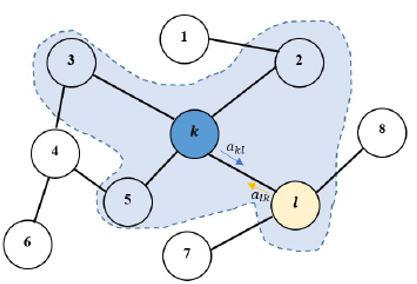
\includegraphics[scale=0.8]{Pic12.JPG}
		\caption{نمایش گرافیکی از یک شبکه تطبیقی با $N=10$ گره}
		\label{p12}
	\end{center}
\end{figure} 


\begin{figure}[h]
	\begin{center}
		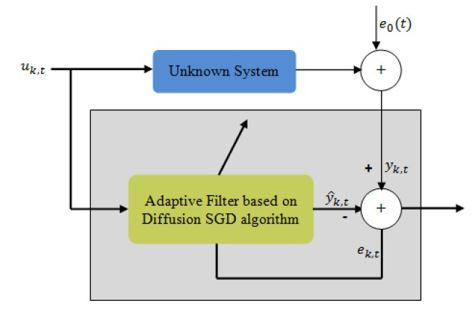
\includegraphics[scale=0.9]{Pic13.JPG}
		\caption{شمای کلی از فیلتر تطبیقی پیشنهادی در یک شبکه تطبیقی توزیع‌شده برای کاربرد شناسایی سیستم}
		\label{p13}
	\end{center}
\end{figure} 

روابط به‌روزرسانی وزن‌ها برای هر عامل $k$ در شبکه تطبیقی توزیع‌شده مبتنی بر الگوریتم گرادیان کاهشی تصادفی مرتبه دوم پس از حل مساله بهینه‌سازی $\min_w\sum_{k=1}^{N}E[\phi(w_ku_k,y_k)]+\frac{\lambda}{2}||w_k||^2_2$ به صورت زیر تعریف می‌شوند:
\begin{equation}\label{e20}
	\begin{cases}
		\psi_{k,t}=w_{k,t-1}-\mu_{t} S_t^{-1} \frac{\partial}{\partial w}[\phi(w_{k,t-1}u_{k,t},y_{k,t})+\frac{\lambda}{2}||w_{k,t-1}||^2_2]\\
		w_{k,t}=\sum_{l\in N_k} a_{lk} \psi_{l,t}
	\end{cases}
\end{equation}
که $\phi(w_{k,t}u_{k,t},y_{k,t})$ تابع زیان گره $k$ در تکرار $t$ است و  با ادغام روابط \textbf{تطبیق} و \textbf{ترکیب} در \ref{e20}، رابطه به‌روزرسانی استفاده شده برای بردار پارامترها $w_{k,t}$ گره $k$ در تکرار $t$ به صورت زیر بدست می‌آید:
\begin{equation}\label{ww}
	w_{k,t}=\sum_{l\in N_k} a_{lk}w_{l,t-1}-\mu_{t} S_t^{-1} \sum_{l\in N_k} a_{lk}(\phi^{'}(w_{l,t-1}^T u_{l,t},y_{l,t})u_{l,t}+\lambda w_{l,t-1})
\end{equation}
الگوریتم یادگیری توزیع‌شده انتشاری پیشنهادی در شبه‌کد \ref{Alg_DSGD} آورده شده است.

\begin{latin}
	

\begin{algorithm}
	\caption{ The ATC Diffusion SGD algorithm}\label{Alg_DSGD}
	\begin{algorithmic}
		\State Initialize $ w_{l,0}=0$ for $l\in\{1,2,...,N\}$
		\State Given non-negative real coefficients \{$a_{l,k}$\} satisfying the conditions in Eq.\ref{e8}
		\State Given suitable step-size parameter $\eta_t>0$
		\For {$t\in\{1,2,...,T\}$}
			\For   {each node $k\in\{1,2,...,N\}$}
				\State Draw example $<\textbf{u}_{k,t},y_{k,t}>\in D$ randomly
				\State Execute the adaptive step of diffusion SGD and Compute $\psi_{k,t}$
				\State Execute the combine step of diffusion SGD and Compute $w_{k,t}$
			\EndFor
		\EndFor
	\end{algorithmic}
\end{algorithm}
\end{latin}

الگوریتم یادگیری توزیع‌شده پیشنهادی در این بخش در حالت کلی و بدون در نظر گرفتن تابع زیان مشخصی معرفی شد. تابع زیان یک تابع ریاضی است که تفاوت بین مقادیر پیش‌بینی شده توسط الگوریتم یادگیری و مقادیر واقعی را کمینه‌سازی می‌کند. در واقع عملکرد الگوریتم یادگیری را اندازه‌گیری می‌کند و فرآیند بهینه‌سازی را با ارائه بازخورد در مورد میران نزدیکی جواب با داده‌ها هدایت می‌کند. توابع خطا مختلفی تا کنون ارائه شده است که هر یک ویژگی‌ها و قابلیت‌های متفاوتی دارد. 

وجود داده‌های پرت و انواع نویز در محیط‌های یادگیری اجتناب ناپذیری است که باعث می‌شوند عملکرد الگوریتم‌های یادگیری توزیع‌شده به شدت کاهش یابد. برخی از توابع خطا در برابر نویزها و داده‌‌های پرت مقاوم نیستند، در نتیجه عملکرد الگوریتم یادگیری را به شدت تحت تاثیر قرار می‌دهند. در بخش بعدی، تعدادی از توابع خطا مناسب حل مسائل رگرسیون معرفی می‌گردند و سپس الگوریتم یادگیری توزیع‌شده مقاوم ارائه می‌شود. 	
\subsection{الگوریتم یادگیری تطبیقی انتشاری مقاوم}
استفاده از توابع زیان مقاوم در برابر نویزهای مختلف محیطی سبب افزایش مقاومت روش یادگیری توزیع‌شده پیشنهادی می‌شود. تابع زیان مربع خطا\footnote{\lr{Square Loss function}}  تنها در برابر نویزهای گاوسی مقاوم است اما در محیط‌های آغشته به نویزهای غیرگاوسی عملکرد ضعیفی دارد و در اکثر مواقع واگرا می شود. توابع زیانی مانند شبه‌هابر\footnote{\lr{Pseudo-Huber}} ، کورانتروپی\footnote{\lr{Correntropy}}  و ... نسبت به نویزهای غیرگاوسی مقاوم می‌باشند. 

تابع زیان ‌هابر برای مقادیر بزرگ خطا $e$ خطی و برای مقادیر کوچک آن از درجه دوم می‌باشد. تابع زیان شبه‌هابر یک تقریب مشتق‌پذیر نرم از تابع زیان هابر می‌باشد که ترکیبی از توابع هزینه مربعی و قدرمطلق است. مزیت اصلی این تابع نسبت به تابع زیان هابر این است که دوبار مشتق‌پذیر و نرم است و نسبت به نویز گاوسی و همچنین نویزهای غیرگاوسی مقاوم می‌باشد.
\begin{equation}
	L_{\delta}(e)=
	\begin{cases}
		\frac{1}{2}e^2\qquad if \quad |e|<\delta\\
		\delta(|e|-\frac{1}{2}\delta)\qquad otherwise
	\end{cases}
	Huber Loss
\end{equation}

\begin{equation}
	L_{\delta}(e)=\delta^2(\sqrt{1+(e/\delta)^2}-1)\qquad Pseudo-Huber Loss
\end{equation}
که $e$ خطا فیلتر و $\delta$ یک پارامتر اضافی برای کنترل شیب در مقادیر بزرگ خطا است. 

تابع زیان کورآنتروپی \cite{CorrEntrop} که در الگوریتم‌های یادگیری تئوری اطلاعات استفاده می‌شود، به صورت زیر تعریف می‌گردد: 
\begin{equation}
	j_k (w)=1-\exp⁡(- \frac{e^2}{2\eta^2})      \qquad Correntropy Loss
\end{equation}

که $\eta$ پارامتر خطا کورآنتروپی می‌باشد که پهنای باند کرنل را تنظیم می‌کند. تایع زیان کورآنتروپی نسبت به داده‌های پرت و نویزهای ضربه‌ای مقاوم است و در محیط‌هایی که دارای نویز غیرگاوسی می‌باشد، بسیار مناسب خواهد بود. این تابع زیان با پهنای باند کمتر، تابع‌ نرم‌تر و نسبت به نویز مقاوم‌تر می‌باشد. 

در مقاله \cite{Barron17} یک تابع زیان کلی مقاوم و تطبیقی معرفی شده است که در واقع تعمیمی از تعدادی تابع زیان از جمله مربع خطا، شبه هابر، \lr{Charbonnier} تعمیم یافته،  \lr{Cauchy/Lorentzian} \cite{CauchyLoss}، \lr{Welsch/Leclerc} \cite{WelschLoss}و \lr{Geman-McClure} \cite{GemanLoss} است. 

\begin{equation}\label{GenralLosses}
	L(e,\alpha,c)=\frac{|\alpha-2|}{\alpha}\left((\frac{(\frac{e}{c})^2}{|\alpha-2|}+1)^{\frac{\alpha}{2}}-1\right) 
\end{equation}
که $\alpha\in \mathbb{R}$ پارامتری برای کنترل مقاومت خطا است و $c>0$ هم یک پارامتر مقیاس برای کنترل اندازه کاسه درجه دوم خطاها در نردیکی $a=0$ است. به ازای $\alpha=2$ و $\alpha=1$ رفتار آن به ترتیب نزدیک به تابع زیان مربع خطا و شبه هابر است. زمانیکه $\alpha\rightarrow 0$، خطا کوشی یا \lr{Cauchy} و $\alpha=-2$ خطای \lr{Gman-McClure} را سبب می‌شود. همچنین زمانیکه $\alpha\rightarrow -\infty$، خطا \lr{Welsch} را خواهیم داشت.  در ادامه روابط این توابع خطا به صورت مجزا آورده شده است.
	\begin{flalign}
	&L(e,c)=1-\exp(-\frac{1}{2}(\frac{e}{c})^2) \qquad Welsch/Leclerc \quad Loss\\
	&L(e,c)=\log(\frac{1}{2}(\frac{e}{c})^2+1) \qquad \quad Cauchy/Lorentzian \quad Loss\\
	&L(e,c)=\frac{2(\frac{e}{c})^2}{(\frac{e}{c})^2+4} \qquad \quad \qquad Geman-McClure \quad Loss
\end{flalign} 
تابع زیان شبه‌هابر مشتق‌پذیر است و نرم‌تر از سایر توابع زیان بوده و نسبت به تابع زیان مربع خطا کمتر به نویز در داده‌های ورودی و داده‌های پرت حساس است. با در نظر گرفتن عواملی چون سادگی، مقاومت در برابر انواع خطاهای محیطی و نرم بودن، تابع زیان شبه‌هابر به عنوان تابع زیان الگوریتم یادگیری پیشنهادی انتخاب می‌شود. بر این اساس، تابع هزینه محلی $J_k(w)$ هر گره $k$ به صورت زیر خواهد بود:

\begin{equation}\label{Jk}
	J_k(w)=\delta^2(\sqrt{1+(\frac{e_k}{\delta})^2}-1)
\end{equation}
تابع هزینه $J_k(w)$  قویا محدب بوده و $\nabla^2J_k(w)$ یک ماتریس هسین مثبت معین است.  مشتق $J_k(w)$ با توجه به $w$ در تکرار $t$ به صورت زیر است:
\begin{equation}\label{deriv_Jk}
	\nabla J_k(w)=-\frac{e_k(t)u_{k,t}^T}{\sqrt{1+(\frac{e_k(t)}{\delta})^2}}
\end{equation}

با جایگذاری \ref{deriv_Jk} در \ref{ww} به عنوان مشتق تابع زیان $\phi$، رابطه به‌روزرسانی بردار پارامترها برای هر گره $k$ در روش یادگیری توزیع‌شده پیشنهادی مبتنی بر تابع زیان شبه‌هابر و براساس استراتژی "تطبیق سپس ترکیب"، به صورت زیر ارائه می‌شود:
\begin{equation}\label{complete_w}
	w_{k,t}=\sum_{l\in N_k}a_{lk}w_{l,t-1}-\mu S^{-1}_t \lambda(\sum_{l\in N_k}a_{lk}w_{l,t-1})+\mu S^{-1}_t (\sum_{l\in N_k}a_{lk}\frac{e_l(t)u_{l,t}^T}{\sqrt{1+(\frac{e_l(t)}{\delta})^2}})
\end{equation}

همانطور که قبلاً ذکر شد، $S^{-1}_t$ به عنوان پیش شرطی است که در صورت انتخاب یک مقدار مناسب برای آن می‌توان نرخ همگرایی الگوریتم را بهبود بخشد. در این رساله، ما $S^{-1}_t$ را با استفاده از رابطه بازگشتی زیر در هر تکرار تعیین می‌کنیم:
\begin{equation}\label{S_inv}
	\begin{cases} 
		S^{-1}_0=\xi I_M\\\\
		Gain_t=\frac{S^{-1}_{t-1} u_{k,t}} {\gamma+u_{k,t}^T S^{-1}_{t-1} u_{k,t}}\\\\
		S^{-1}_t=S^{-1}_t - Gain_t u^T_{k,t} S^{-1}_t
	\end{cases}
\end{equation}
که $\xi$ یک مقدار ثابت است و $I_M$ نشان‌دهنده یک ماتریس همانی به ابعاد $M \times M$ است. $S_t^{-1}$ برای هر نمونه ورودی یا هر دسته داده ورودی در هر تکرار به روز می‌شود. در صورت وارد شدن نویز به داده‌های خروجی، مدل داده با اعمال نویز به صورت

\begin{equation}\label{modelee}
	d_k (t)=w_o^T u_k (t)+\nu_k (t)
\end{equation}

 است. در این مدل داده، ترم $\nu_k (t)$ نشان‌دهنده یک فرآیند نویز افزاینده با میانگین صفر یا همان نویز سفید گوسی است که مستقل از داده‌های ورودی $u_k (t)$ است. الگوریتم یادگیری توزیع‌شده مقاوم پیشنهادی \lr{RDSGD} (\lr{Robust DiffusionSGD}) در شبه‌کد \ref{Alg_RDSGD} آورده شده است. 
\begin{latin}
	

	\begin{algorithm}
	\caption{The ATC form of RDSGD algorithm}\label{Alg_RDSGD}
	\begin{algorithmic}
		\State Parameters: $\lambda$, $0<\gamma<1$, $\mu>0$
		\State Initialization: $ w_{k,0}=0$ for $l\in\{1,2,...,N\}$
		\State Set the coefficients \{$a_{l,k}$\} based on the conditions in Eq.\ref{e8}
		\For {$t\in\{1,2,...,T\}$}
			\For   {each node $k\in\{1,2,...,N\}$}
				\State Draw sample $(\textbf{u}_{k,t},y_{k,t})$ randomly
				\State Estimation error: \\\qquad$e_k(t)=d_k(t)-w_{k,t-1}^T\textbf{u}_{k,t}$
				\State Adaptive step: \\\qquad$\psi_{k,t}=w_{k,t-1}-\mu_k S_t^{-1}\left(\lambda w_{k,t-1}-\frac{e_k(t)\textbf{u}_{k,t}^T}{\sqrt{1+(\frac{e_k(t)}{\delta})^2}}\right)$
				\State Combination step: \\\qquad$w_{k,t}=\sum_{l\in N_k}a_{lk}\psi_{l,t}$
			\EndFor
		\EndFor
	\end{algorithmic}
\end{algorithm}
\end{latin}

\subsection{کاربرد الگوریتم یادگیری پیشنهادی در مساله پیش‌بینی}
یکی از کاربردهای مهم این الگوریتم پیشنهادی، مساله پیش‌بینی است. در این رساله توانایی الگوریتم یادگیری را در پیش‌بینی داده‌های بورس ایران مورد ارزیابی قرار خواهیم داد. روابط پیشنهادی برای مدل کردن مساله پیش‌بینی به صورت زیر می‌باشند:
\begin{equation}
	\begin{cases}
		\hat{d}_k(t)=w_{k,t}^T\dot{d_k (t:-1:t-M)}\\
		e_k(t)=d_k(t+1)-\hat{d}_k(t)
	\end{cases}
\end{equation}

\begin{equation}
	\begin{cases}
		\psi_{k,t}=w_{k,t-1}-\mu S^{-1}(\lambda w_{k,t-1}+\frac{d_k(t:-1:t-M)^T e_k(t)}{\sqrt{1+(\frac{e_k(t)}{\delta})^2}})\\
		w_{k,t}=\sum_{l\in N_k}a_{lk}\psi_{l,t}
	\end{cases}
\end{equation}

\section{رویکرد یادگیری توزیع‌شده پیشنهادی}

در این بخش به معرفی رویکرد یادگیری توزیع‌شده پیشنهادی که متناسب با خصوصیات شبکه‌های تطبیقی توزیع‌شده است با جزئیات پرداخته می‌شود. همان‌طور که قبلا هم اشاره شده است، رویکرد پیشنهادی در دو مرحله اصلی برون‌خط و برخط اجرا می‌شود. شکل \ref{p14} نمودار جریان کلی رویکرد یادگیری پیشنهادی را نشان می‌دهد. هما‌ن‌طور که دیده می‌شود، مرحله برون‌خط که مرحله پیش‌پردازش نیز نامیده می‌شود، شامل دو بخش رصد کردن\footnote{\lr{Monitoring}} شبکه و منطقه‌بندی\footnote{\lr{Regioning}} شبکه است. در بخش رصد کردن شبکه به محاسبه توان پردازشی هر گره پرداخته می‌شود. بدین منظور یک دسته‌داده با اندازه ثابت به هر گره داده می‌شود و زمان انجام آن محاسبه می‌شود. سپس زمان‌های بدست آمده نرمال خواهند شد. در بخش منطقه‌بندی شبکه، خوشه‌بندی گره‌ها براساس فاصله گره‌ها از همدیگر، توان پردازشی محاسبه‌شده در بخش قبلی و میزان اعتماد بین گره‌ها انجام خواهد شد. در مرحله برخط، فرایند یادگیری موازی مبتنی بر مدل محاسباتی پیشنهادی \lr{BSP} فدرالی (\lr{FBSP}) بر روی شبکه تطبیقی توزیع‌شده که در مرحله پیش‌پردازش منطقه‌بندی شده است، اجرا خواهد شد.
\begin{figure}[h]
	\begin{center}
		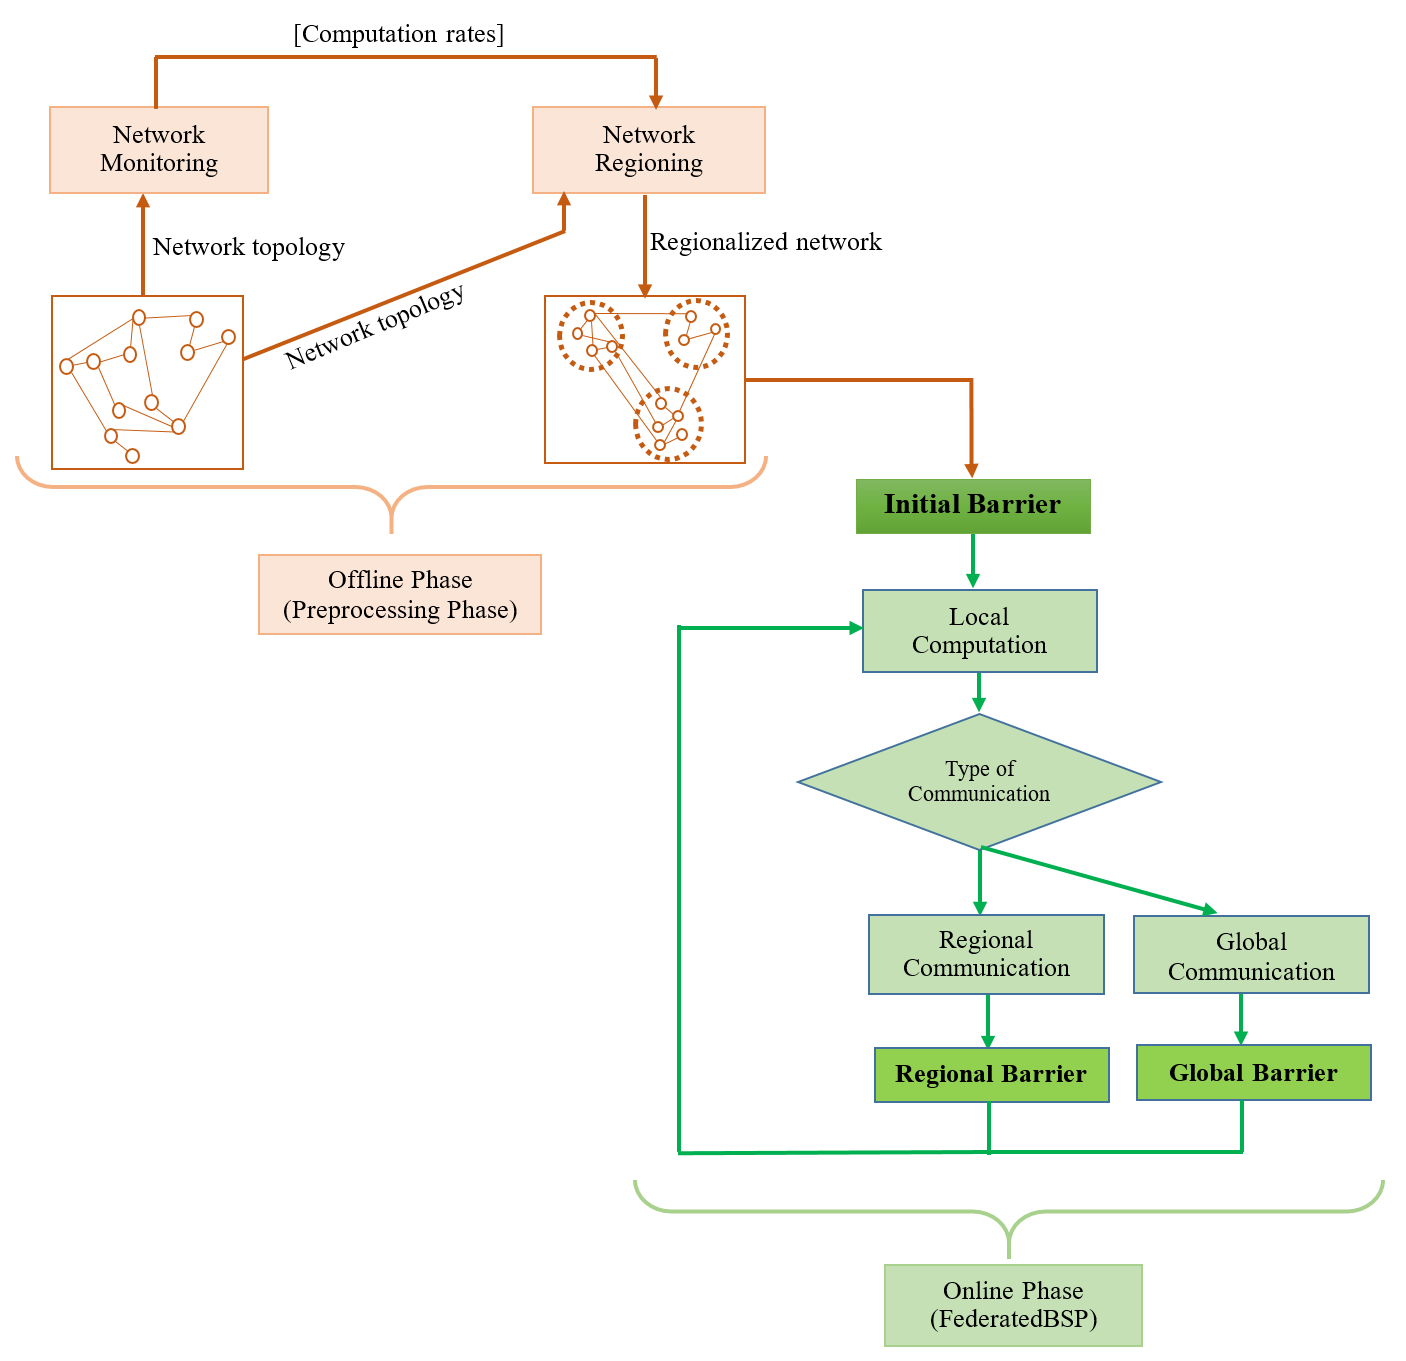
\includegraphics[scale=0.7]{Pic16.png}
		\caption{نمودار جریان رویکرد یادگیری پیشنهادی}
		\label{p14}
	\end{center}
\end{figure} 

\subsection{مدل محاسباتی پیشنهادی \lr{BSP} فدرالی یا \lr{FBSP}}
مدل محاسباتی \lr{BSP} فدرالی (\lr{FBSP}) همانند مدل محاسباتی \lr{BSP} از سه بخش مهم محاسبه، ارتباط و همگام‌سازی مانعی تشکیل شده است. با این تفاوت که بر اساس منطقه‌بندی انجام شده و همسایگی گره‌ها در شبکه، دو نوع ارتباط بین گره‌های شبکه شامل \textbf{ارتباط منطقه‌ای} و \textbf{ارتباط سراسری} در مدل \lr{BSP} فدرالی معرفی شده است. در ارتباط منطقه‌ای، هر گره با گره‌های همسایه‌اش در منطقه‌ای که قرار دارد ارتباط برقرار می‌کند و تبادل داده بین‌ آنها انجام می‌شود. در ارتباط سراسری، هر گره با گره‌های همسایه‌اش در کل شبکه ارتباط برقرار می‌کند و تبادل داده بین‌ آنها انجام می‌شود. به دنبال نوع ارتباط‌های متفاوت در مدل محاسباتی پیشنهادی، دو نوع همگام‌سازی مانعی شامل \textbf{همگام‌سازی مانعی منطقه‌ای} و \textbf{همگام‌سازی مانعی سراسری} معرفی شده است. همگام‌سازی مانعی منطقه‌ای بین گره‌های همسایه واقع در یک منطقه و همگام‌سازی مانعی سراسری بین گره‌های همسایه واقع در کل شبکه انجام خواهد شد. این کار سبب می‌شود میزان ارتباطات بین گره‌ها در زمان اجرا کاهش یابد و از رخ دادن مساله کندکننده‌ها جلوگیری شود. 

مساله کندکننده‌ها به یکی از دو دلیل 1) وجود گره‌های کند در بین گره‌های شبکه و 2) عدم توازن بار در بین گره‌‌ها، رخ خواهد داد. در صورتی که محیط توزیع‌شده یک محیط ناهمگن باشد، احتمال حضور گره‌های کند در شبکه بسیار بالا است که این موضوع افزایش زمان انتظار گره‌های سریع‌تر را نتیجه خواهد داد. در حالتی که داد‌ه‌های پردازشی در شبکه توزیع‌شده از نوع ویدیو یا هر داده دیگری با اندازه‌های متفاوت باشد، عدم توازن بار را در گره‌ها خواهیم داشت که سبب می‌شود برخی از گره‌ها با اندازه داده یا اندازه ویدیو کوچک‌تر محاسبات‌شان زودتر تمام شود که باید منتظر سایر گره‌ها برای اتمام کارشان بماند. در نتیجه زمان انتظار افزایش پیدا خواهد کرد. 

همان‌طور که قبلا هم اشاره شده است، همگام‌سازی یا مکانیزم کنترل مانع بین گره‌ها از اجزای مهم طراحی رویکردهای یادگیری توزیع‌شده است. مکانیزم‌های همگام‌سازی کنترل مانع به طور کلی به سه مکانیزم غیرهمگام (\lr{ASP})، همگام با کهنگی (\lr{SSP}) و همگام مانعی (\lr{BSP}) دسته‌بندی می‌شوند. شکل \ref{p17} مکانیزم همگام‌ مانعی پیشنهادی در مدل محاسباتی \lr{BSP} فدرالی را با روش‌های دیگر بر اساس معیارهای دقت همگرایی و توان عملیاتی آموزش (معکوس زمان اجرا تکرارها) مقایسه می‌کند.

\begin{figure}[h]
	\begin{center}
		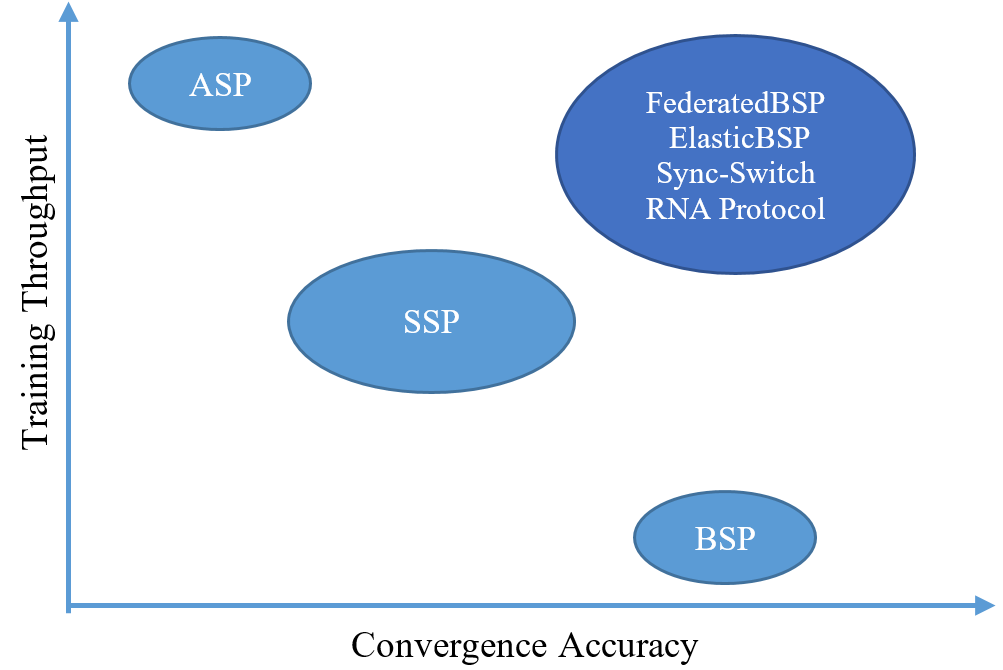
\includegraphics[scale=0.7]{Comp1.PNG}
		\caption{مقایسه مکانیزم همگام‌سازی مانعی پیشنهادی با سایر مکانیزم‌ها}
		\label{p17}
	\end{center}
\end{figure}

\subsection{مرحله رصد کردن شبکه}
مرحله رصد کردن به صورت یک مرحله برون‌خط و یک عملیات پیش‌پردازشی برای محاسبه توان کاری یا نرخ محاسباتی هر گره اجرا می‌شود. بدین منظور، توسط یک گره مرکزی به سایر گره‌ها در شبکه یک دسته داده با اندازه ثابت ارسال می‌شود. هر گره‌ پس از پردازش دسته داده، گرادیان محاسبه شده را به گره مرکزی ارسال می‌کند. بر این اساس گره مرکزی نرخ محاسباتی هر گره، میانگین زمان پردازش تمام گره‌های شبکه و سریع‌ترین و کندترین گره‌ها را مشخص می‌کند و این اطلاعات را به منظور منطقه‌بندی شبکه به مرحله بعدی ارسال می‌کند. 
در این مرحله بعد از محاسبه نرخ محاسباتی گره‌ها، اندازه دسته داده هر گره به صورت ضریبی از نرخ محاسباتی آن گره تعیین می‌گردد. به عبارتی، به گره‌های سریع‌تر اندازه دسته‌های بزرگتر و به گره‌های کندتر اندازه دسته‌های کوچک‌تری تخصیص داده می‌شود. این کار سبب می‌شود که زمان انتظار گره‌ها در زمان همگام‌سازی مانعی سراسری و همچنین میزان کهنگی پارامترهای مدل در بخش ارتباطات تا حدودی کاهش یابد و زمان محاسبه گره‌ها با نرخ‌های محاسباتی متفاوت نزدیک بهم شود. 


\subsection{مرحله منطقه‌بندی شبکه}
توپولوژی شبکه به صورت یک گراف ویژگی $G=(V,E,A)$ در نظر گرفته می‌شود، به‌طوریکه در آن $V$  مجموعه گره‌های شبکه، \lr{E} مجموعه یال‌های موجود بین گره‌ها و \lr{A} مجموعه خصوصیات هر گره را نشان می‌دهد. به هر گره $v_i\in V$ یک بردار ویژگی شامل نرخ پردازش محاسباتی گره $cp_i$ و ضرایب وزن همسایگی گره$[a_{1i},a_{2i},...,a_{ni}]$ تخصیص داده می‌شود. منطقه‌بندی گره‌های شبکه باید به صورتی انجام شود که هر کدام از منطقه‌ها علاوه‌بر نزدیکی ساختاری و وزن همسایگی، از لحاظ محتوایی نیز بهم شبیه باشند. بدین منظور در این مرحله، ابتدا گره‌ها بر اساس نرخ پردازش محاسباتی $cp_i$ و میانگین نرخ پردازش محاسباتی کل گره‌های شبکه $\bar{CP}$ ، برچسب‌گذاری می‌شوند. سپس از روش خوشه‌بندی ساختاری-محتوایی به نام \lr{ICS-cluster } \cite{Kesh2020} استفاده می‌شود. در این روش ابتدا ساختار و محتوای گراف اولیه ترکیب شده و یک گراف ساختاری-محتوایی ساخته می‌شود. وزن شباهت گره‌ها با استفاده از رابطه \ref{e21} محاسبه می‌شود. وزن شباهت گره‌های $i$ و $j$ که با $WS_{ij}$ نشان داده می‌شود به عنوان وزن یال بین آنها در گراف ساختاری-محتوایی ایجاد شده در نظر گرفته خواهد شد.

\begin{equation}\label{e21}
	WS_{ij}=a\times (\frac{1}{Dist(i,j)})+b\times Sim(i,j)+c*a_{ij}
\end{equation}

که $i\notin j$ است و $a$ ضریب شباهت ساختاری، $b$ ضریب شباهت محتوایی و $c$ ضریب وزن همسایگی میان گره $i$ و $j$ است. این ضرایب در فرآیند یادگیری مقدارشان تعیین می‌گردد. وزن همسایگی نشان‌دهنده میزان اطمینان و اهمیت اطلاعات دریافتی از گره همسایه است. مقدار $Sim(i,j)$ را با استفاده از معیارهای مختلف اندازه‌گیری شباهت همچون ضریب شباهت ژاکارد\footnote{\lr{Jaccard similarity}}  می‌توان محاسبه کرد. برای محاسبه شباهت ساختاری از عکس فاصله دو گره از یکدیگر استفاده می‌شود. در این رابطه هر چه فاصله دو گره بیشتر باشد، شباهت ساختاری کمتر خواهد بود. فاصله بین دو گره می‌تواند فاصله واقعی آنها از یکدیگر باشد یا برابر با تعداد یال‌های بین آنها در شبکه در نظر گرفته شود. به طور کل فاصله بین گره‌ها از طریق الگوریتم دایجسترا\footnote{\lr{Dijkstra algorithm}}  محاسبه می‌شود. 

بعد از محاسبه وزن‌های شباهت، میانگین این وزن‌ها $\bar{WS}$ در کل شبکه به عنوان یک حد آستانه برای ایجاد گراف ساختاری-محتوایی استفاده می‌شود. اگر $WS_{ij}$ از مقدار $\bar{WS}$ بیشتر باشد، بین دو گره $i$ و $j$ در گراف مورد نظر یالی رسم می‌شود. در غیر این صورت بین آن دو گره هیچ یالی در نظر گرفته نخواهد شد.

در گراف وزن‌دار حاصل، ابتدا هر گره به عنوان یک منطقه در نظر گرفته می‌شود. سپس به ترتیب گره‌هایی که یال‌های با وزن بالا دارند با یکدیگر ادغام شده و تشکیل یک منطقه را می‌دهند. تمام گره‌هایی که با چند یال به منطقه‌ای متصل هستند، به یک یال تبدیل شده و از وزن آن‌ها میانگین گرفته می‌شود و به عنوان وزن ارتباط آن گره با منطقه در نظر گرفته می‌شود. این فرآیند به صورت تکراری تا جایی ادامه می‌یابد که تعداد منطقه‌ها برابر با تعداد منطقه‌های موردنظر شوند. در فرآیند منطقه‌بندی با اعمال شرطی بر روی اندازه منطقه‌ها در زمان اجرا، متعادل‌سازی اندازه منطقه‌ها در نظر گرفته می‌شود. شکل \ref{p115} نمودار جریان الگوریتم خوشه‌بندی ساختاری-محتوایی مورد نظر را نشان می‌دهد که گراف اولیه و ماتریس شباهت ورودی‌های نمودار جریان و گراف خوشه‌بندی شده با تعداد خوشه‌های مورد نظر خروجی آن می‌باشند. به عنوان یک مثال برای واضح‌تر شدن روند کار این الگوریتم، در شکل \ref{p15} مراحل خوشه‌بندی ساختاری-محتوایی بر روی یک شبکه با ماتریس شباهت گره‌های آن نمایش داده شده است.
\begin{figure}[h]
	\begin{center}
		
		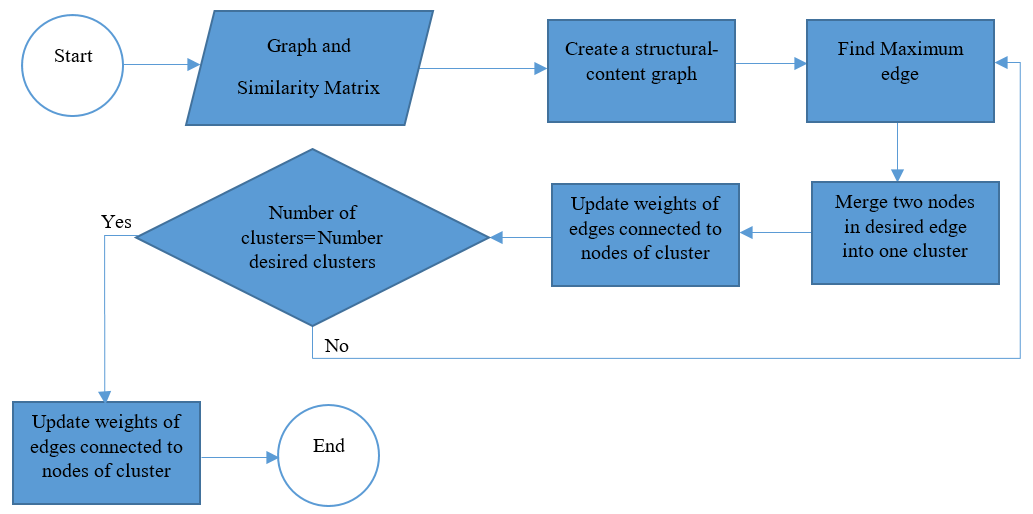
\includegraphics[scale=0.8]{icsCluster.PNG}
		\caption{نمودار جریان الگوریتم خوشه‌بندی ساختاری-محتوایی}
		\label{p115}
	\end{center}
\end{figure}

\begin{figure}[h]
	\begin{center}
		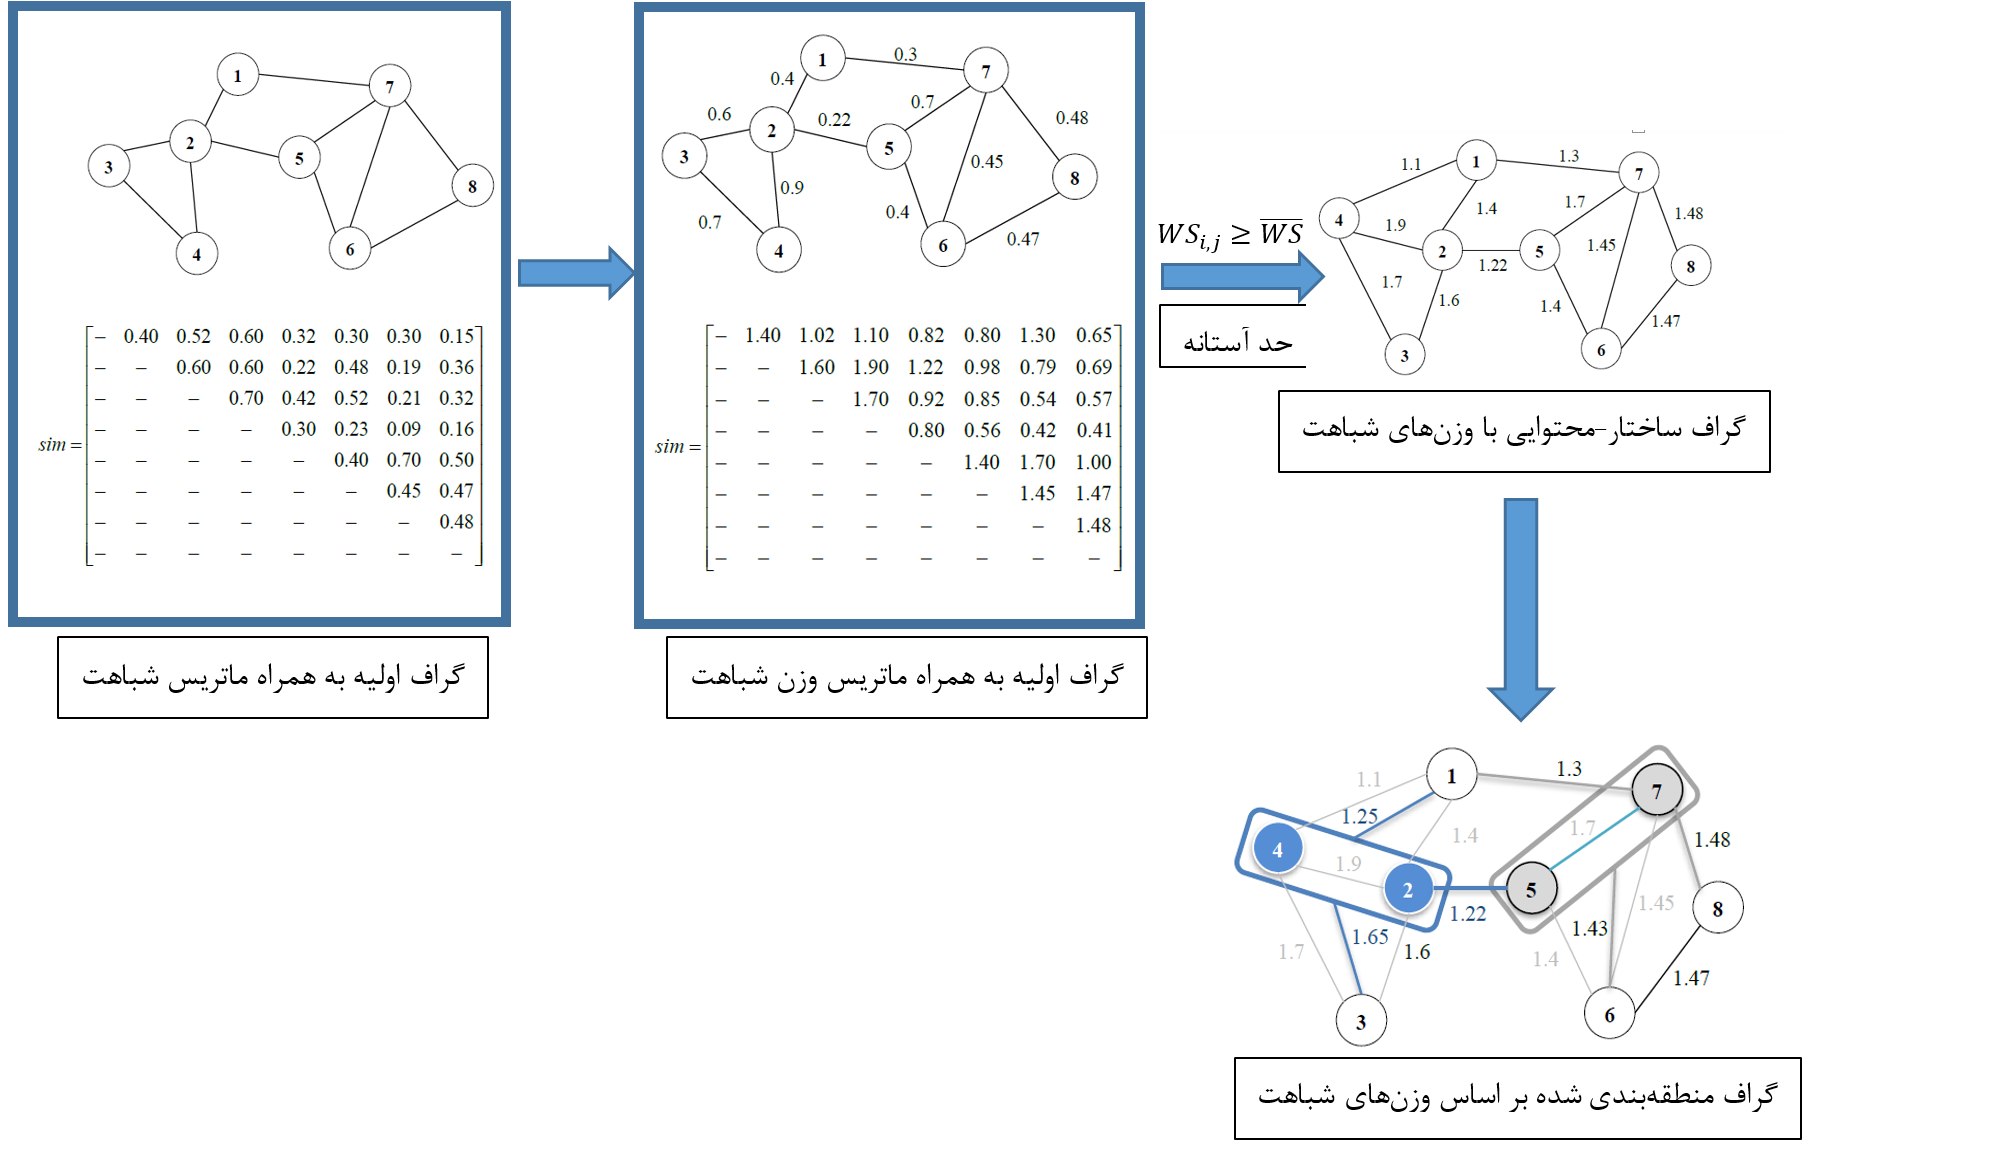
\includegraphics[scale=0.45]{Graph1.png}
		\caption{مراحل اجرای الگوریتم خوشه‌بندی  ساختاری-محتوایی بر روی یک شبکه}
		\label{p15}
	\end{center}
\end{figure}

\subsection{مرحله برخط رویکرد یادگیری پیشنهادی }
مرحله برخط رویکرد یادگیری پیشنهادی مبتنی بر مدل محاسباتی توسعه‌یافته \lr{BSP} فدرالی است و رفتار شماتیکی این مرحله در شکل \ref{p16} با بیان جزئیات نشان داده شده است. در این نمودار جریان، هر ستون یک گره (پردازنده) را نشان می‌دهد که گره‌ها به صورت مستقل و موازی اقدام به مقداردهی اولیه کپی بردار پارامتر خودشان می‌کنند و یک دسته داده از داده‌های محلی خود متناسب با نرخ پردازشی محاسبه شده در مرحله پیش‌پردازش نیز انتخاب می‌کند. 
\begin{figure}[h]
	\begin{center}
		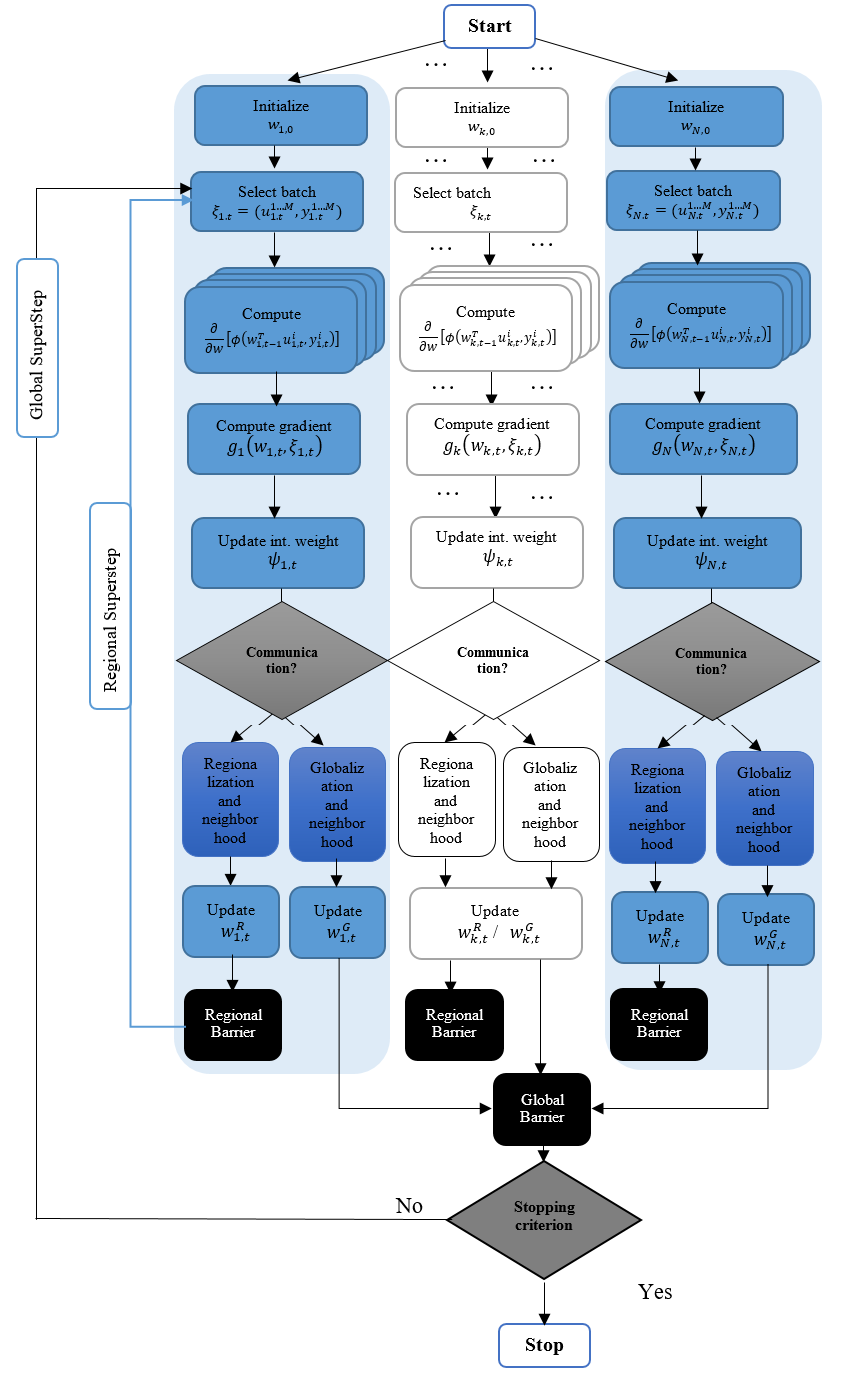
\includegraphics[scale=0.6]{Flow1.png}
		\caption{رفتار شماتیکی مرحله برخط رویکرد پیشنهادی مبتنی بر مدل محاسباتی توسعه یافته \lr{BSP} فدرالی}
		\label{p16}
	\end{center}
\end{figure}

بعد از محاسبه گرادیان محلی و به‌روزرسانی بردار پارامتر میانی، هر گره در مورد نوع ارتباط با گره‌های همسایه‌اش در شبکه باید تصمیم‌گیری نماید. در صورت انتخاب ارتباط منطقه‌ای با گره‌های همسایه، بردار پارامتر به صورت منطقه‌ای با بردارهای پارمتر همسایه‌ها در همان منطقه ترکیب و سپس به‌روزرسانی می‌گردد. در انتهای هر تکرار منطقه‌ای، یک همگام‌سازی مانعی منطقه‌ای نیز باید اجرا گردد. این مراحل یک ابرگام منطقه‌ای در مدل محاسباتی \lr{BSP} فدرالی را تشکیل می‌دهند. اگر گره ارتباط سراسری را انتخاب کند، بردار پارامتر به صورت سراسری با بردارهای پارامتر همسایه‌ها در کل شبکه ترکیب و سپس به‌روزرسانی می‌گردد. در انتهای هر تکرار سراسری، یک همگام‌سازی مانعی سراسری نیز باید اجرا گردد. این مراحل یک ابرگام سراسری در مدل محاسباتی \lr{BSP} فدرالی را تشکیل می‌دهند. این مرحله از رویکرد پیشنهادی کمک می‌کند تا یک پیاده‌سازی موازی غیرهمگام در شبکه‌های تطبیقی توزیع‌شده داشته باشیم. 


با فرض داشتن یک شبکه کوچک کاملا متصل شامل 5 گره با قدرت‌های پردازشی متفاوت، تفاوت زمان‌های انتظار گره‌های کند و سریع و مساله کندکننده‌ها به وضوح در دو حالت اعمال همگام‌سازی مانعی سراسری و همگام‌سازی مانعی منطقه‌ای که به ترتیب در شکل‌های \ref{p18-1} و \ref{p18-2} نشان داده شده است. در شکل \ref{p18-1} گره \lr{C} که سریع‌ترین گره از لحاظ قدرت پردازشی است، مدت زیادی باید منتظر بماند تا عملیات محاسباتی در کندترین گره به پایان برسد. در حالیکه در شکل \ref{p18-2} که همگام‌سازی مانعی منطقه‌ای اعمال شده است، مدت زمان انتظار گره \lr{C} کاهش می‌یابد. در نتیجه مجموع زمان انتظار در کل شبکه نیز در هر بار اجرای همگام‌سازی مانعی کاهش خواهد یافت. همچنین در مدت زمان مشخص، توان عملیاتی و کار انجام شده توسط رویکرد پیشنهادی با روش منطقه‌بندی بیشتر است. در حالتی‌که هیچ منطقه‌بندی در شبکه اجرا نشود، کار انجام شده به اندازه سه ابرگام سراسری است. در مقابل در همان مدت زمان، در حالتی‌که منطقه‌بندی در شبکه اجرا شود، کار انجام شده در یک منطقه به اندازه سه ابرگام و در منطقه دیگر به اندازه 5 ابرگام است.

\begin{figure*}[ht]
	\centering
	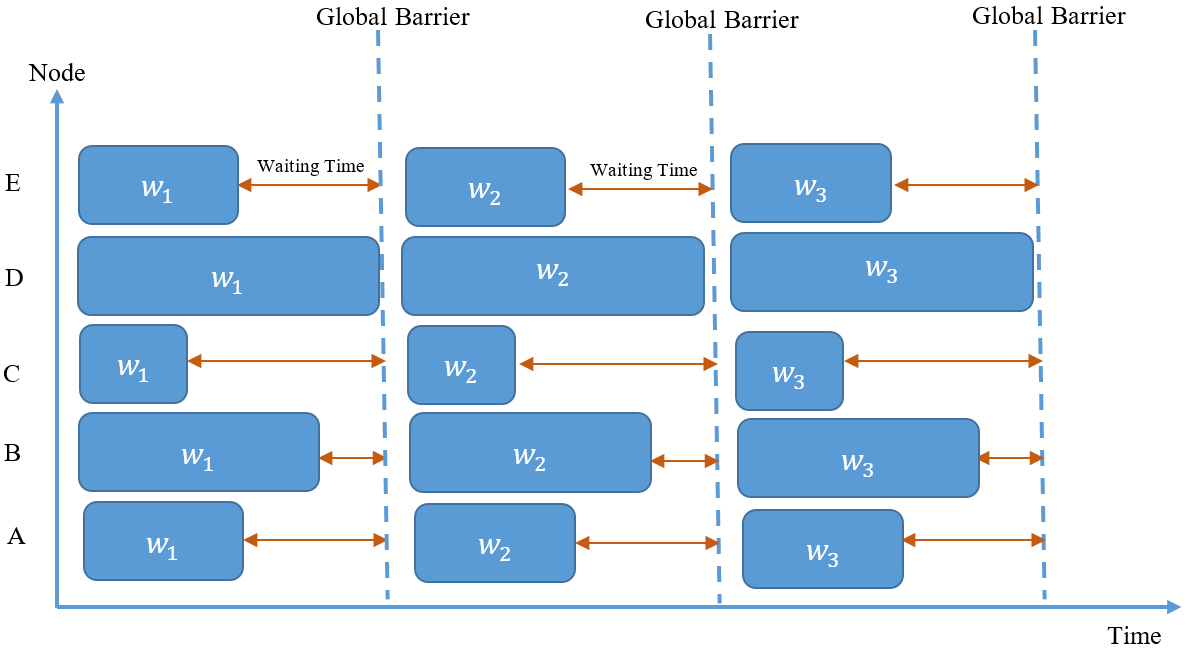
\includegraphics[width=.8\linewidth]{Pic20.PNG}  
	\caption{همگام‌سازی مانعی سراسری و تاثیر آن بر زمان انتظار کل شبکه}
	\label{p18-1}
\end{figure*}

\begin{figure*}[ht]
	\centering 
	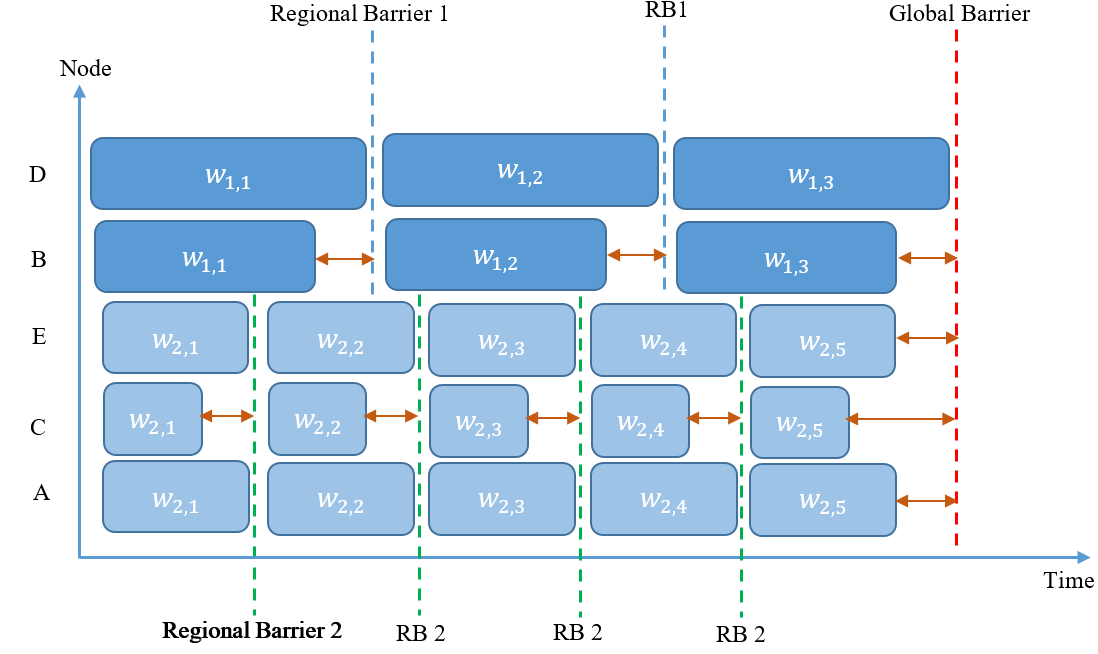
\includegraphics[width=.8\linewidth]{Pic21.PNG}  
	\caption{همگام‌سازی مانعی منطقه‌ای و تاثیر آن بر زمان انتظار کل شبکه}
	\label{p18-2}
\end{figure*}

شکل \ref{p20-2} مراحل اجرای مدل محاسباتی \lr{BSP} فدرالی از دیدگاه گره \lr{N1} در شبکه منطقه‌بندی شده \ref{p20-1} را نشان می‌دهد. ارتباطات گره \lr{N1} با همسایگانش با یال‌های نارنجی رنگ مشخص شده‌اند. در حالت ارتباط منطقه‌ای گره \lr{N1} با گره‌های \lr{N2 } و \lr{N3 } ارتباط برقرار می‌کند و با دریافت بردارهای وزن میانی گره‌های مذکور و ترکیب آنها بردار وزن $w_{1t}^R$ خود را به صورت منطقه‌ای به‌روزرسانی می‌کند و سپس همگام‌سازی مانعی منطقه‌ای اجرا خواهد شد. بعد از اجرای چندین ابرگام منطقه‌ای و احراز شرایط اجرای ارتباط سراسری، گره \lr{N1 } با گره‌های \lr{N2}، \lr{N3}، \lr{N4} و \lr{N5} ارتباط برقرار می‌کند و با دریافت بردارهای وزن میانی گره‌های مذکور و ترکیب آنها اقدام به به‌روزرسانی بردار وزن $w_{1t}^G $ خود به صورت سراسری می‌کند و سپس همگام‌سازی مانعی سراسری اجرا خواهد شد.
\begin{figure*}[ht]
	\centering
	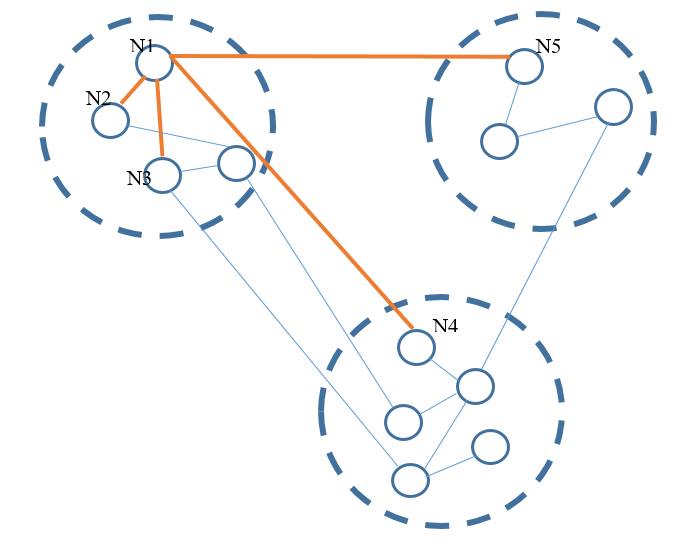
\includegraphics[width=.6\linewidth]{Pic22.PNG}  
	\caption{یک شبکه منطقه‌بندی‌شده}
	\label{p20-1}
\end{figure*}

\begin{figure*}[ht]
		\centering
		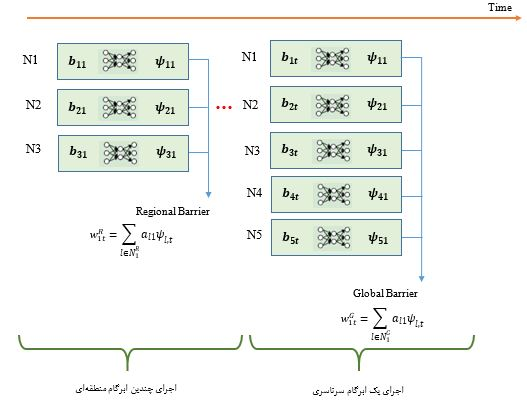
\includegraphics[width=1\linewidth]{Pic23.PNG}
		\caption{مثالی از نحوه اجرای ارتباطات و همگام‌سازی مانعی منطقه‌ای و  سراسری در شبکه \ref{p20-1}}
	\label{p20-2}
\end{figure*}

\subsection{مدل سیستم و فرمول‌بندی مساله}
	در این بخش مدل کلی سیستم یادگیری توزیع‌شده، تابع هدف و فرضیاتی که بر روی تابع هدف در نظر گرفته شده است را تعریف می‌کنیم. 
	در یک سیستم یا به عبارتی در یک شبکه از گره‌ها، مجموعه‌ای‌ از منطقه‌ها به نام \lr{$\mathcal{R}$} تعریف می‌شود که $\mathcal{R}=\{1,...,R\}$ است. هر منطقه $r\in \mathcal{R}$ شامل مجموعه‌ای از گره‌ها $M^{(r)}$ است که $|M^{(r)}|=N^{(r)}$. مجموعه تمام گره‌ها در کل شبکه به صورت $M=\bigcup_{r=1}^R M^{(r)}$ تعریف می‌شود. گره‌ها از طریق یک گراف ارتباطی متصل غیرجهت‌‌دار $G=(M,E)$ با یکدیگر در ارتباط می‌باشند. هر گره $i$ یک مجموعه داده آموزشی محلی $U^{(i)}$ دارد که کل مجموعه داده‌های آموزشی سیستم به صورت $U=\bigcup_{i=1}^N U^{(i)}$ تعریف می‌شود.  
	
	فرض کنید $N_i=\{j|e_{ij}\in E\}$ مجموعه همسایگی گره $i$ در گراف $G$ و $N_i^{(r)}=\{j| e_{ij}\in E\quad and\quad j\in M^{(r)}\}$ مجموعه همسایگی گره $i$ در منطقه $r$ است. هر گره $i\in M^{(r)}$ می‌تواند با هر گره‌ همسایه $ k$ در منطقه $r$ ($k\in N_i^{(r)}$) و هر گره همسایه $j$ در شبکه $G$ ($j\in N_i$) ارتباط برقرار کند. 
  
	
	همان‌طور که قبلا بیان شده است، $w\in R^{M\times 1}$ بردار وزن یا بردار پارامترها نامیده می‌شود و هدف ما پیدا کردن $w$ است به گونه‌ای که تابع هدف زیر بر روی مجموعه داده‌های آموزشی مورد نظر کمینه گردد:
\begin{equation}
	J(w)=\frac{1}{|U|}\sum_{U^i\in U} J_i(w,U^i)
\end{equation}
	
که $J_i(.)$ تابع زیان است. هر گره‌ با همکاری سایر گره‌های همسایه خود سعی در کمینه کردن این تابع زیان با استفاده از مجموعه داده‌های آموزشی محلی خود دارد. 
	
	در هر تکرار، هر گره دسته‌ای از داده‌های آموزشی محلی خود را به صورت تصادفی نمونه‌برداری می‌کند. فرض کنید که $\xi$ دسته نمونه‌برداری شده و $g(w;\xi)=\frac{1}{|\xi|}\sum_{u^i\in \xi} \nabla f(w;u^i)$ گرادیان دسته‌ای است. برای سادگی در ادامه $g(w)$ به جای $g(w;\xi)$ به کاربرده می‌شود.
	
	
\begin{assumption}
	در این رساله فرضیات زیر در مورد تابع هدف و گرادیان دسته‌ای در نظر گرفته شده است:
		\begin{enumerate}\label{Farz1}
		\item \label{F11}
		تابع هدف $J: R^M\rightarrow R$ پیوسته و مشتق‌پذیر است و گرادیان آن از قانون لیپشیتز با ثابت $\delta>0$ پیروی می‌کند که
		\begin{center}
			$||\nabla_{w}J(w_2)-\nabla_{w}J(w_1)||_2<=\delta||w_2-w_1||_2, \qquad for\quad all\quad w_1,w_2\in R^{M\times 1}$
		\end{center}
		این شرط مستلزم این است که گرادیان‌ها خیلی سریع تغییر نکنند. 
		\item \label{F12}
		در حالت کلی تابع هدف $J(w) $ کران پایین دارد. این فرض مستلزم این است که تابع هدف با مقدار $J_{inf} (w)$ از پایین محدود باشد.
		
		\begin{center}
			$J(w)\ge J_{inf}(w)>-\infty \qquad for \quad all \quad w\in R^{M\times 1}$
		\end{center}
		
		\item \label{F13}
		گرادیان‌های دسته‌ای $g(w)$ بی‌طرفانه هستند:	
		\begin{center}
			$E_{\xi|w}[g(w)]=\nabla J(w) \qquad for \quad all \quad w\in R^{M\times 1}$ 
		\end{center} 
		\item \label{F14}
		با فرض اینکه اسکالرهای $\sigma$ و $\beta$ وجود دارند که 
		
		\begin{center}
			$E_{\xi|w} ||g(w)-\nabla J(w)||_2^2\le \beta||\nabla J(w)||_2^2+\sigma^2,\qquad for \quad all \quad w\in R^{M\times 1}$  
		\end{center}
	این فرض شبیه فرض واریانس محدود شده است. در مورد آخر فرض می‌شود که داده‌های محلی در هر گره می‌توانند به عنوان یک تخمین بی‌طرفانه برای مجموعه داده کامل با همان واریانس محدود استفاده شوند. این فرضیات در تحلیل همگرایی الگوریتم‌های گرادیان کاهشی تصادفی رایج و معمول هستند.
\end{enumerate}
\end{assumption}

رابطه به‌روزرسانی استفاده شده در مرحله تطبیق و ترکیب هر گره‌ $K$ و نرخ‌ متفاوت محاسبات (قدرت پردازشی متفاوت) گره‌ها به صورت زیر مدل می‌شود:

\begin{flalign}\label{ATC1}
	&\psi_{k,t}=w_{k,t-1}-\mu_k(t) S_t^{-1}(\lambda\ w_{k,t-1}-\nabla_{w}{J_k(w)})\\
	&w_{k,t}=\sum_{l\in N_k} a_{lk} \psi_{l}(t)\\
	&\mu_k(t)=
	\begin{cases}
		\mu_k\quad with\ a\ probability\ of\ P_k\\
		0\ \quad with\ a\ probability\ of\ 1-P_k
	\end{cases}
\end{flalign} 
که هر گره $k$، از $\tau$ تکرار تنها $\tau^{(k)}$  تکرار را اجرا می‌کند ($\tau^{(k)} \leq \tau$). $P$ یک بردار به طول $N$ است که $P_k=\frac{\tau^{(k)}}{\tau}$ احتمال اینکه گره $k$ یک گام به‌روزرسانی را در هر تکرار اجرا نماید. 

تحلیل ما در این بخش بر چگونگی تکامل مدل‌ گره‌ها متمرکز است. ابتدا یک فرمول معادل از الگوریتم پیشنهادی از نظر تکامل مدل‌ گره‌ها ارائه کرده و سپس نتیجه اصلی را در مورد همگرایی و پایداری الگوریتم خود ارائه می‌کنیم. رفتار سیستم با استفاده از قانون به‌روزرسانی کلی \ref{mo} مدل می‌شود:	

\begin{equation}\label{mo}
	w_t=B(t) w_{t-1}-\mu(t) S_t^{-1}\lambda\ B(t) w_{t-1} +\mu(t)S_t^{-1}\ B(t) G_t
\end{equation}
که $G_t=[\nabla J_1(t), \nabla J_2(t), ..., \nabla J_N(t)]^T$،   $w_t=[w_{1,t},w_{2,t}, ..., w_{N,t}]^T$ و    $B(t)\in R^{N\times N}$ یک عملگر متغیر با زمان است که دو مدل ارتباط سراسری و ارتباط منطقه‌ای در رویکرد پیشنهادی را شامل می‌شود. به منظور مدل کردن رفتار سیستم با یک رابطه به‌روزرسانی کلی، ماتریس $B(t)$ را به صورت زیر تعریف می‌کنیم:
\begin{equation}\label{Bmarix}
	B(t)=
	\begin{cases}
		Z(t)\quad if\ t\ mod \ q=0\\
		V(t)\quad otherwise
	\end{cases}
\end{equation}
در مرحله ارتباطات سراسری که هر گره برای به‌روزرسانی بردار پارامتر خود با همسایگانش در کل شبکه ارتباط برقرار می‌کند، ماتریس مربعی $Z(t)$ به ابعاد $N\times N$ به صورت $Z=A$ در نظر گرفته می‌شود. در مرحله ارتباطات منطقه‌ای که هر گره برای به‌روزرسانی بردار پارامتر خود با همسایگان هم‌منطقه‌اش ارتباط برقرار می‌کند، ماتریس مربعی $V(t)$ به ابعاد $N\times N$ به گونه‌ای تعریف می‌شود که هر درایه این ماتریس، وزن گره‌های همسایه و هم‌منطقه با گره  $i$ را نشان می‌دهد. 
\begin{equation}\label{Nt}
	Z_{i,j}(t)=
	\begin{cases}
		a_{ij}\quad if\ j\in N_i\\
		0 \quad otherwise
	\end{cases},\quad
	V_{i,j}(t)=
	\begin{cases}
		a_{ij}\quad if\ j\in N_i^{(r)}\\
		0 \quad otherwise
	\end{cases}
\end{equation}

فرض کنید $\boldsymbol{\Xi}=\{\xi_1{(t)},...,\xi_N{(t)}\}$ مجموعه دسته داده‌های استفاده شده توسط $N$ عامل در زمان $t$ باشد. بدون از دست دادن کلیت، ما یک دسته داده  به هر عامل اختصاص می‌دهیم، حتی اگر عامل موردنظر در یک تکرار عمل به‌روزرسانی را اجرا نکند. همچنین مجموعه متغیرهای تصادفی برنولی $\boldsymbol{\Theta}=\{\theta_1(t),...,\theta_N(t)\}$ به صورت زیر تعریف می‌شوند: 
\begin{equation}\label{eTheta}
	\theta_i(t)=
	\begin{cases}
		1\qquad with\quad probability\quad p_i\\
		0\qquad with\quad probability\quad (1-p_i)
	\end{cases}
\end{equation}
بر این اساس، می‌توان تعریف معادلی برای گرادیان $g_i(t)$ به صورت زیر ارائه داد: 


\begin{equation}
	g_i(t)=\theta_i(t)g(\xi_i(t))
\end{equation}
در ادامه برای سادگی به جای $E_{\boldsymbol{\Theta}_t,\boldsymbol{\Xi}_t|W_t}$ از معادل آن $E_t$ در روابط استفاده می‌شود. بر اساس فرض \ref{F13} در \ref{Farz1} خواهیم داشت:
\begin{equation}
	E_t[g_i(t)]=p_i E[g(w_i(t))]\\
	=p_i\nabla J(w_i(t))
\end{equation}
و همچنین زمانی‌که $i\ne j$ باشد، خواهیم داشت:

\begin{equation}
	E_t[(g_i(t))^T g_j(t)]=p_i p_j E_t[g(w_i(t))]^T E_t[g(w_j(t))]=p_i p_j \nabla J{(w_i(t))}^T \nabla J(w_j(t))
\end{equation}

بر اساس فرض شماره \ref{F14} در \ref{Farz1} می‌توان نتیجه گرفت که، 
\begin{flalign}
	E_t[\lVert(g_i(t))-&\nabla J(w_i(t))\rVert^2]= E_t[\lVert(g_i(t))\rVert^2+\lVert \nabla J(w_i(t))\rVert^2 -2 (g_i(t))^T \nabla J(w_i(t))]\\
	&=E_t[\lVert(g_i(t))\rVert^2+\lVert \nabla J(w_i(t))\rVert^2 -2 E_t[(g_i(t))]^T \nabla J(w_i(t))]\\
	&=p_i E_t[\lVert(g(w_i(t)))\rVert^2+\lVert \nabla J(w_i(t))\rVert^2 -2 p_i E_t[(g(w_i(t)))]^T \nabla J(w_i(t))]
\end{flalign}

\begin{flalign}
	\begin{split}
		E_t[\lVert(g_i(t))-&\nabla J(w_i(t))\rVert^2]=p_i E_t[\lVert(g(w_i(t)))\rVert^2+ p_i \lVert \nabla J(w_i(t))\rVert^2\\
		&-2 p_i E_t[(g(w_i(t)))]^T \nabla J(w_i(t))]+ (1-p_i) \lVert \nabla J(w_i(t))\rVert^2
	\end{split}\\
	&=p_i E_t[\lVert(g(w_i(t)))-\nabla J(w_i(t))\rVert^2+ (1-p_i) \lVert \nabla J(w_i(t))\rVert^2\\
	&\le p_i \beta \lVert \nabla J(w_i(t))\rVert^2+p_i\sigma^2 + (1-p_i) \lVert \nabla J(w_i(t))\rVert^2\\
	&= (p_i (\beta-1)+1) \lVert \nabla J(w_i(t))\rVert^2+p_i\sigma^2
\end{flalign}
	

\section{الگوریتم رویکرد یادگیری پیشنهادی}
الگوریتم \ref{Alg_Proposed} شبه‌کد کلی بخش یادگیری رویکرد پیشنهادی را نشان می‌دهد. هر گره یک کپی از مدل یا همان بردار پارامترها را در اختیار دارد. گره‌ها در هر منطقه به صورت موازی و مستقل از سایر منطقه‌های شبکه آموزش می‌بینند و مدل خود را با کمک گره‌های همسایه در منطقه خود به‌روزرسانی می‌کنند. همچنین، گره‌ها قادر هستند مدل خود را با کمک گره‌های همسایه در کل شبکه به صورت دوره‌ای به‌روزرسانی کنند.
\begin{latin}
	\begin{algorithm}
	\caption{ The algorithm of proposed approach}\label{Alg_Proposed}
	\begin{algorithmic}[1]
		\State Initialize $ w_{l}(0)=0$ for $l\in\{1,2,...,N\}$
		\State Given non-negative real coefficients \{$a_{lk}$\}
		\State Given suitable step-size parameter $\mu_t>0$
		\For {$t\in\{1,2,...,T\}$}
		\For  {$r\in  \mathcal{R}$} 
		\For {$k\in M^{(r)}$}
		\For {$j\in \{t, t+1, ..., t+\tau-1\}$}
		\State $\psi_{k,t}=w_{k,t-1}-\mu_k(t) S_t^{-1}(\lambda w_{k,t-1}-\nabla_{w}{J_k(w)})$
		\EndFor
		\If{$t\ mod\ q!=0$}
		\State $w_{k,t}=\sum_{l\in N_k^{(r)}} a_{lk} \psi_{l,t}$
		\Else
		\State $w_{k,t}=\sum_{l\in N_k} a_{lk} \psi_{l,t}$
		\EndIf
		\EndFor
		\EndFor
		\EndFor
	\end{algorithmic}
\end{algorithm}
\end{latin}
	
\section{تجزیه و تحلیل نظری الگوریتم پیشنهادی}
با تمرکز بر جنبه‌های عددی الگوریتم \lr{DSGD}، برای تحلیل و اثبات همگرایی الگوریتم یادگیری پیشنهادی از شیوه ارائه شده در مقاله \cite{Zin2010} که برای الگوریتم‌های گرادیان کاهشی تصادفی مرتبه دوم است، الهام گرفته شده است و همچنین از سنجه جدید اختلاف همگرایی وزنی \footnote{\lr{the weighted convergence difference}} استفاده شده است. این سنجه با استفاده از رابطه \ref{DeltaW} تعریف می‌شود. 

\begin{equation}\label{DeltaW}
	\Delta(w_{k,t},w_{k,t-1},w)=R_{w,t,k}-R_{w,t-1,k}=\lvert\lvert w_{k,t}-w\rvert\rvert^2_S-\lvert\lvert w_{k,t-1}-w\rvert\rvert^2_S
\end{equation}

در این بخش همگرایی الگوریتم یادگیری پیشنهادی در حالت کلی و بدون در نظر گرفتن یک تابع زیان خاص مورد بررسی قرار می‌گیرد. برای سادگی $\phi^{'}(w_{k,t}^T u_{k,},y_{k,t})$ به صورت مختصر با $\phi^{'}_{k,t}$ نمایش داده می‌شود. همان طور که ذکر شد، سنجه اختلاف همگرایی وزنی اساس تحلیل ما است و به صورت زیر تجزیه می‌شود:

\begin{equation}\label{decompositionF}
	\begin{split}
		&\Delta(w_{k,t},w_{k,t-1},w)=\\
		& \lvert\lvert\sum_{l\in N_k} a_{lk}w_{l,t-1}-\mu_{t} S^{-1} \sum_{l\in N_k} a_{lk}\left(\phi^{'}_{l,t}u_{l,t}+\lambda w_{l,t-1}\right)-w\rvert\rvert^2_S-\\
		&\lvert\lvert\sum_{l\in N_k} a_{lk}w_{l,t-2}-\mu_{t-1} S^{-1} \sum_{l\in N_k} a_{lk}\left(\phi^{'}_{l,t-1}u_{l,{t-1}}+\lambda w_{l,t-2}\right)-w\rvert\rvert^2_S
	\end{split}
\end{equation}

که 

\begin{equation}\label{decomposition}
	\begin{split}
		&\Delta(w_{k,t},w_{k,t-1},w)=\lvert\lvert\sum_{l\in N_k} a_{lk}w_{l,t-1}-w\rvert\rvert^2_S+\\
		&\mu^2_t \lvert\lvert\sum_{l\in N_k} a_{lk}\phi^{'}_{l,t}u_{l,t}+\lambda \sum_{l\in N_k} a_{lk} w_{l,t-1}\rvert\rvert^2_{S^{-1}}-\\
		&2\mu_t \left(\sum_{l\in N_k} a_{lk}w_{l,t-1}-w\right)^T\left(\sum_{l\in N_k} a_{lk}\phi^{'}_{l,t}u_{l,t}+\lambda \sum_{l\in N_k} a_{lk} w_{l,t-1}\right)\\
		&-\lvert\lvert\sum_{l\in N_k} a_{lk}w_{l,t-2}-w\rvert\rvert^2_S+2\mu_{t-1}\left(\sum_{l\in N_k} a_{lk}w_{l,t-2}-w\right)^T\\
		&\left(\sum_{l\in N_k} a_{lk}\phi^{'}_{l,t-1}u_{l,t-1}+\lambda \sum_{l\in N_k} a_{lk} w_{l,t-2}\right)\\
		&-\mu^2_{t-1}\lvert\lvert\sum_{l\in N_k} a_{lk}\phi^{'}_{l,t-1}u_{l,{t-1}}+\lambda \sum_{l\in N_k} a_{lk} w_{l,t-2}\rvert\rvert^2_{S^{-1}}
	\end{split}
\end{equation}
در هر تکرار $t$، بردار پارامترهای بدست آمده $w_{k,t}$ باید نسبت به بردار پارامترهای تکرار قبلی $w_{k,t-1}$، به بردار پارامترهای بهینه $w$ نزدیک‌تر شود. برای خلاصه‌سازی تجزیه بدست آمده در \ref{decomposition}، جملات $\lvert\lvert\sum_{l\in N_k} a_{lk}w_{l,t-1}-w\rvert\rvert^2_S+\mu^2_t \lvert\lvert\sum_{l\in N_k} a_{lk}\phi^{'}_{l,t}u_{l,t}+\lambda \sum_{l\in N_k} a_{lk} w_{l,t-1}\rvert\rvert^2_{S^{-1}}$ و $||\sum_{l\in N_k} a_{lk}w_{l,t-2}-w||^2_S+\mu^2_t||\sum_{l\in N_k} a_{lk}\phi^{'}_{l,t-1}u_{l,{t-1}}+\lambda \sum_{l\in N_k} a_{lk} w_{l,t-2}||^2_{S^{-1}}$ به ترتیب با $A^2$ و $B^2$, نمایش داده می‌شوند. 
\begin{theorem}
	با فرض استقلال نمونه‌های یادگیری $<u_{k,t},y_{k,t}>k=1,...,N, t=1,...,T$ و ثابت بودن اندازه گام‌ها در تکرارهای مختلف $\mu_{t}=\mu$ و $\lambda\ge0$، با استفاده از تجزیه انجام شده در \ref{decomposition} و تعریف سنجه اختلاف همگرایی وزنی داریم:
	\begin{equation}\label{inequality}
		\begin{split}
			&\Delta(w_{k,t},w_{k,t-1},w)\leq A^2-\\
			&2\mu (\lambda \left[\lVert\sum_{l\in N_k} a_{lk}w_{l,t-1}-\frac{1}{2}w\rvert\rvert^2_2-\lvert\lvert\sum_{l\in N_k} a_{lk}w_{l,t-2}-\frac{1}{2}w\rvert\rvert^2_2\right]\\
			&+[\left(\sum_{l\in N_k}a_{l,k}\phi^{'}_{l,t}u_{l,t}\right)^T\left(\sum_{l\in N_k}a_{l,k}w_{l,t-1}-w\right)\\
			&-\left(\sum_{l\in N_k}a_{l,k}\phi^{'}_{l,t-1}u_{l,t-1}\right)^T\left(\sum_{l\in N_k}a_{l,k}w_{l,t-2}-w\right)])
		\end{split}
	\end{equation}
	
\end{theorem}

\begin{proof}
	با مرتب‌سازی جملات در رابطه \ref{inequality} و اعمال تغییر نام‌های مورد نظر، رابطه زیر را می‌توانیم بدست آوریم:
	\begin{equation}\label{Eq12}
		\begin{split}
			&\Delta(w_{k,t},w_{k,t-1},w)=A^2-B^2-\\
			&2\mu\lambda \left[\lVert\sum_{l\in N_k} a_{lk}w_{l,t-1}-\frac{1}{2}w\rvert\rvert^2_2-\lvert\lvert\sum_{l\in N_k} a_{lk}w_{l,t-2}-\frac{1}{2}w\rvert\rvert^2_2\right]\\
			&-2\mu\left(\sum_{l\in N_k}a_{l,k}\phi^{'}_{l,t}u_{l,t}\right)^T\left(\sum_{l\in N_k}a_{l,k}w_{l,t-1}-w\right)\\
			&+2\mu\left(\sum_{l\in N_k}a_{l,k}\phi^{'}_{l,t-1}u_{l,t-1}\right)^T\left(\sum_{l\in N_k}a_{l,k}w_{l,t-2}-w\right)
		\end{split}	
	\end{equation}
	جملات با ضرایب $2\mu\lambda$ و $2\mu$ در \ref{Eq12} را می‌توان به ترتیب با $D$ و $E$ نام‌گذاری و خلاصه کرد و رابطه 
	\begin{equation}\label{equality}
		\Delta(w_{k,t},w_{k,t-1},w)=A^2-B^2-2\mu\lambda D-2\mu E
	\end{equation}
	را بدست آورد. به وضوح مشخص است که جمله $B^2$  غیرمنفی است. بر این اساس، رابطه \ref{equality} به صورت نامساوی \ref{inequality2} بازنویسی می‌شود. این نامساوی نتیجه مهم این تحلیل است. 
	\begin{equation}\label{inequality2}
		\Delta(w_{k,t},w_{k,t-1},w)\leq A^2-2\mu (\lambda D+ E)
	\end{equation}
\end{proof}

بسته به سرعت تغییر $\Delta(w_{k,t},w_{k,t-1},w)$، تغییر ممکن است به صورت تدریجی یا ناگهانی باشد. تغییر تدریجی $\Delta(w_{k,t},w_{k,t-1},w)$ باعث می‌شود که نرم‌کننده کمتر تحت تأثیر نویز قرار گیرد. در واقع نرم‌کننده تبدیل به یک کاهنده می‌شود و نرخ همگرایی کاهش می‌یابد. فرض کنید $\mu^*=\argminA_{\mu} \Delta(w_{k,t},w_{k,t-1},w)$. به عبارت دیگر، اگر $\mu^{*}$ منجر به کاهش نرخ همگرایی شود، پس $w_t$ کمتر تحت تاثیر نویز قرار می‌گیرد. در طراحی الگوریتم \lr{DSGD}، اگر بخواهیم الگوریتم سریع‌تر به سمت $w$ حرکت کند، پس باید $\mu^*=\argmaxA_{\mu} \Delta(w_{k,t},w_{k,t-1},w)$ باشد. در این حالت $w_t$ شدیدا به نویز حساس خواهد بود. 

با رشد رابطه \ref{ww}، مقدار عبارت $D$ یک مقدار مثبت کوچک می‌شود. همچنین بخش مشابه آن در عبارت $\theta=A^2-B^2$ نیز یک مقدار مثبت کوچک است. در حالت همگرایی، فاصله بین بردار پارامتر $w$ و $w_{t}$  باید کمتر از فاصله بین  $w$ و $w_{t-1}$ باشد. بنابراین، سمت راست رابطه \ref{inequality} منفی است. عبارت $\lambda D+E$ به $\gamma$  تغییر نام داده می‌شود. همیشه $\theta-2\mu \gamma\le 0$ خواهد بود. با فرض تغییر تدریجی بردار پارامترها، همگرایی الگوریتم \lr{DSGD} در صورت برقراری شرط $\mu \le \frac{\theta}{2\gamma}$ صورت می‌گیرد. 
\begin{assumption}\label{assumption0}
	برای دست یافتن به هدف اصلی و سادگی تحلیل، فرضیات زیر بر روی توابع خطا در نظر گرفته می‌شوند:
	\begin{itemize}
		\item تابع زیان $\phi(\hat{y},y)$ محدب است
		\item ثوابت غیرمنفی $A$ و $B$ به گونه‌ای وجود دارند که $(\phi^{'}(\hat{y},y))^2\leq A\phi(\hat{y},y)+B$
	\end{itemize} 
\end{assumption}

توابع زیانی از جمله هابر، حداقل مربع خطا و ... این فرض را ارضا می‌کنند. به عنوان مثال تابع زیان حداقل مربعات خطا $\phi(\hat{y},y)=(\hat{y}-y)^2$ در حل مساله رگرسیون با انتخاب  $A=4$ و $B=0$  فرض موجود در \ref{assumption0} را ارضا می‌کند. 
برای تحلیل همگرایی الگوریتم \lr{DSGD}،  $\lambda=0$  انتخاب می‌شود. اگر $t\rightarrow\infty$، مساله به کمترین ریسک و خطا همگرا خواهد شد. کران همگرایی به طور مستقیم از نتایج رابطه \ref{inequality} حاصل می‌شود. 

\begin{assumption}\label{Assumption00}
	به منظور تحلیل نرخ همگرایی الگوریتم یادگیری، فرض $\sup\lvert\lvert u_{k,t}\rvert\rvert_{S^{-1}}\leq M$ بر روی هر نمونه داده و برای هر $k=1, 2, ..., N$ و $t=1, 2, ..., T$ در نظر گرفته می‌شود. 
\end{assumption}

\begin{theorem}\label{Theorem00}
	در صورت برقراری فرضیات \ref{assumption0} و \ref{Assumption00} بر روی توابع خطا و نمونه‌های داده، همچنین برای هر گره $k$ در تکرار $t$ فرض می‌کنیم که $\lvert a_{l,k}\rvert\leq L$ برقرار است، پس
	\begin{equation}\label{eq6}
		\begin{split}
			&\Delta(w_{k,t},w_{k,t-1},w)\leq \\
			&\lvert\lvert \sum_{l\in N_k}{a_{l,k}w_{l,t-1}-w} \rvert\rvert^2_S+\mu^2_t \left[(A\sum_{l\in N_k}\phi_{l,t} +B)N_kM^2L^2\right]\\
			&-2\mu_t M\left[(\sum_{l\in N_k}a_{l,k}\phi^{'}_{l,t})^T(\sum_{l\in N_k}a_{l,k}w_{l,t-1}-w)\right]\\
			&+2\mu_t M\left[(\sum_{l\in N_k}a_{l,k}\phi^{'}_{l,t-1})^T(\sum_{l\in N_k}a_{l,k}w_{l,t-2}-w)\right]
		\end{split}
	\end{equation}
\end{theorem}

\begin{proof}
	همان‌طور که قبلا اشاره شد، ضرایب $a_{lk}$ وزن‌های غیرمنفی هستند که شرط در \ref{condition} را ارضا می‌کنند. در نتیجه، $0\leq L\leq 1$ است. برای یافتن یک کران برای جمله دوم $A^2$ در سمت راست رابطه \ref{inequality}، از نامساوی \lr{Cauchy–Schwarz} که به صورت $(\sum x_i y_i)^2\leq \sum x_i^2 \sum y_i^2$ است، استفاده می‌کنیم. بنابراین، می‌توان این جمله را به صورت نامساوی زیر ساده کرد: 
	\begin{equation*}
		\begin{split}
			\lVert\sum_{l\in N_k} a_{lk}\phi^{'}_{l,t}u_{l,t}\rvert\rvert^2&\leq \sum_{l\in N_k}\lvert\lvert a_{l,k}\phi^{'}_{l,t}\rvert\rvert^2 \sum_{l\in N_k}\lvert\lvert u_{l,t}\rvert\rvert^2\\
			&\leq N_k M^2 L^2\sum_{l\in N_k}\lvert\lvert \phi^{'}_{l,t}\rvert\rvert^2\\
			&\leq N_k M^2 L^2(A\sum_{l\in N_k}\phi_{l,t}+B)
		\end{split}
	\end{equation*}
	که $N_k$ مجموعه همسایگی گره $k$ است. جمله $D$ به دلیل $\lambda=0$ حذف خواهد شد. یک کران برای جمله $E$ در رابطه \ref{inequality} بر اساس نامساوی \lr{Cauchy–Schwarz} به صورت زیر بدست می‌آید:
	\begin{equation*}
		\begin{split}
			E&\leq M\left[(\sum_{l\in N_k}a_{l,k}\phi^{'}_{l,t})^T(\sum_{l\in N_k}a_{l,k}w_{l,t-1}-w)\right]\\
			&-M\left[(\sum_{l\in N_k}a_{l,k}\phi^{'}_{l,t-1})^T(\sum_{l\in N_k}a_{l,k}w_{l,t-2}-w)\right]
		\end{split}
	\end{equation*}
\end{proof}

قضیه \ref{Theorem00} یک کران بالا برای خطا تولید شده توسط رابطه به‌روزرسانی بردار پارامترها نتیجه می‌دهد و نشان می‌دهد که همگرایی الگوریتم \lr{DSGD} وابسته به پارامتر اندازه گام $\mu$ است. 

به منظور سادگی بحث، جملات سمت راست رابطه \ref{inequality}، به $A_c=N_kM^2L^2(A\sum_{l\in N_k}\phi_{l,t} +B)$،   $B_c=M[(\sum_{l\in N_k}a_{l,k}\phi^{'}_{l,t})^T(\sum_{l\in N_k}a_{l,k}w_{l,t-1}-w)-(\sum_{l\in N_k}a_{l,k}\phi^{'}_{l,t-1})^T(\sum_{l\in N_k}a_{l,k}w_{l,t-2}-w)]$ و $C_c=\lvert\lvert \sum_{l\in N_k}{a_{l,k}w_{l,t-1}-w} \rvert\rvert^2_S$ تغییر نام داده می‌شوند. 

\begin{theorem}
	با فرض تغییرات تدریجی بردارهای پارامتر هر گره $k$ در هر تکرار $t$ و تحت تاثیر فرضیات \ref{assumption0} و \ref{Assumption00} و $\mu_t=\mu>0$، پارامتر اندازه گام الگوریتم یادگیری \lr{DSGD} در بازه زیر اعمال می‌شود: 
	\begin{equation}\label{cond_eta}
		\frac{B_c-\sqrt{B_c-A_cC_c}}{A_c}<\mu_t<\frac{B_c+\sqrt{B_c-A_cC_c}}{A_c}
	\end{equation}
\end{theorem}

\begin{proof}
	سمت راست رابطه \ref{inequality} به صورت $f(\mu)=A_c\mu^2 -2\mu B_c+C_c$ بازنویسی می‌شود که این رابطه یک معادله درجه دوم با متغیر نامشخص $\mu$ و ضرایب مشخص $A_c$، $B_c$ , $C_c$ است. به منظور همگرا شدن الگوریتم، این معادله باید غیرمثبت باشد.
	\begin{equation}\label{fmu}
		A_c\mu^2 -2\mu B_c+C_c\leq 0
	\end{equation}
	غیرمنفی بودن $A_c$ و $C_c$ واضح است. پس لازم است بر روی $B_c$ برای تعیین علامت معادله درجه دوم بحث کنیم. اگر $B_c<0$ و $\Delta=4B_c^2-4A_cC_c<0$ یا $\Delta=0$ باشد، علامت معادله درجه دو مشابه علامت $A_c$ است. همان طور که قبلا اشاره شده است، $A_c$ همیشه غیرمنفی است که بر خلاف شرط مورد نظر برای همگرایی است. اگر $\Delta>0$ باشد، علامت معادله درجه دوم بین دو ریشه $\mu_1=\frac{B_c-\sqrt{B_c-A_cC_c}}{A_c}$ و  $\mu_2=\frac{B_c+\sqrt{B_c-A_cC_c}}{A_c}$ مخالف علامت $A_c$ است. طبق فرض $B_c<0$،  شرط \ref{cond_eta}  برای دستیابی به همگرایی باید ارضا شود. همانطور که قبلاً فرض کردیم، پارامتر اندازه گام $\mu>0$ است. بنابراین، 
	\begin{equation}
		0<\mu<\frac{B_c+\sqrt{B_c-A_cC_c}}{A_c}
	\end{equation}
	
\end{proof}

همانطور که در این بخش دیده شد، همگرایی الگوریتم یادگیری توزیع‌شده پیشنهادی در حالت کلی و بدون در نظر گرفتن تابع زیان مشخصی بررسی و اثبات شد. تابع زیان یک تابع ریاضی است که تفاوت بین مقادیر پیش‌بینی شده توسط الگوریتم یادگیری و مقادیر واقعی را کمینه‌سازی می‌کند. در واقع عملکرد الگوریتم یادگیری را اندازه‌گیری می‌کند و فرآیند بهینه‌سازی را با ارائه بازخورد در مورد میزان نزدیکی جواب با داده‌ها هدایت می‌کند. توابع خطا مختلفی تا کنون ارائه شده است که هر یک ویژگی‌ها و قابلیت‌های متفاوتی دارد. 

\section{تجزیه و تحلیل نظری رویکرد پیشنهادی}
به منظور تجزیه و تحلیل کارایی رویکرد پیشنهادی، بردار گرادیان \ref{deriv_Jk} بر اساس دو جمله اول سری مک‌لوران به صورت زیر  تقریب زده می‌شود:

\begin{equation}\label{grad_j}
	\nabla J_k(w)\cong-u_{k,t}^T e_k(t)+ \frac{1}{\delta^2}u_{k,t}^T e_k^3(t)
\end{equation}
بردارهای وزن خطای محلی هر گره $k$ به صورت \ref{WEV} تعریف می شوند:

\begin{flalign}\label{WEV}
	&\tilde{w}_{k,t}=w_o-w_{k,t}\\
	&\tilde{\boldsymbol{\psi}}_{k,i}=w^o-\boldsymbol{\psi}_{k,i}
\end{flalign}

با جایگذاری مدل در نظر گرفته شده برای سیگنال مطلوب $d_k(t)$ (\ref{modelee}) در رابطه بردار خطا تخمین $e_k(t)=d_{k,t}-w_{k,t-1}^T u_{k,t}$ و در نظر گرفتن \ref{WEV}، تعریف $e_k(t)$ به صورت زیر بازنویسی می‌شود:

\begin{equation}\label{e_k}
	\begin{split}
		e_k(t)&=u_{k,t}^T(w_o-w_{k,t-1})+\nu_k(t)\\
		&=u_{k,t}^T \tilde{w}_{k,t-1}+\nu_k(t)
	\end{split}
\end{equation}
جمله $e_k^3(t)$ در \ref{grad_j} بر اساس عبارت $e_k(t)e^2_k(t)$ و \ref{e_k} به صورت \ref{e3} نوشته می‌شود.
\begin{equation}\label{e3}
	\begin{split}
		e_k^3(t)&=(u_{k,t}^T\tilde{w}_{k,t-1})^3+3\nu_k(t)(u_{k,t}^T\tilde{w}_{k,t-1})^2\\
		&+3\nu_k^2(t)(u_{k,t}^T\tilde{w}_{k,t-1})+\nu_k^3(t)
	\end{split}
\end{equation}
با جایگذاری رابطه بدست آمده برای  $e^3_k(t)$ در \ref{grad_j} و در نظر گرفتن بردار وزن خطای محلی در \ref{WEV}، رابطه $\tilde{w}_{k,t}$ به صورت زیر حاصل می شود:
\begin{equation}\label{w_vector}
	\begin{split}
		\tilde{w}_{k,t}&=\sum_{l\in N_{k,t}}b_{lk} \tilde{w}_{k,t-1}-\mu S^{-1}\sum_{l\in N_{k,t}}b_{lk}(u_{k,t}u^T_{k,t}\tilde{w}_{k,t-1})\\
		&-\mu S^{-1} \sum_{l\in N_{k,t}}b_{lk} u^T_{k,t} \nu_k(t)\\
		&+\mu S^{-1}\frac{a}{2\delta^2}\sum_{l\in N_{k,t}}b_{lk}  u^T_{k,t}\{(u_{k,t}^T\tilde{w}_{k,t-1})^3+3\nu_k(t)(u_{k,t}^T\tilde{w}_{k,t-1})^2
		\\
		&+3\nu_k^2(t)(u_{k,t}^T\tilde{w}_{k,t-1})+\nu_k^3(t)\}+\mu \lambda S^{-1} \sum_{l\in N_{k,t}}b_{lk} w_{k,t-1}
	\end{split}
\end{equation}
که مجموعه همسایگی $N_{k,t}$ با توجه به رابطه \ref{Nt} و مقدار $t$  توسط یکی از مجموعه های $N_k$ یا $N_k^{(r)}$ مقداردهی می‌شود. $b_{lk}$ درایه $lk$ ماتریس $B(t)$  است. به منظور سادگی تحلیل رویکرد پیشنهادی، تعریف بردارها و ماتریس‌های زیر را خواهیم داشت: 
\begin{flalign}\label{Q1}
	&\mathcal{R}_{k,t} \overset{\Delta}{=}  u_{k,t}^T u_{k,t}\\
	&\mathcal{G}_{k,t} \overset{\Delta}{=}  u_{k,t}^T \nu_k(t)\\
	&\mathcal{P}^{'}_{k,t} \overset{\Delta}{=}  u_{k,t}^T (u_{k,t}^T \tilde{w}_{k,t-1})^3\\
	&\mathcal{Q}^{'}_{k,t} \overset{\Delta}{=}  \nu_k(t) u_{k,t} (u_{k,t}^T \tilde{w}_{k,t-1})^2\\
	&\mathcal{H}_{k,t} \overset{\Delta}{=} \nu_k(t) u_{k,t}^T u_{k,t}\\
	&\mathcal{S}_{k,t} \overset{\Delta}{=} \nu^2_k(t) u_{k,t}^T u_{k,t}\\
	&\mathcal{T}_{k,t} \overset{\Delta}{=}  u_{k,t}^T \nu^3_k(t)	
\end{flalign}
هنگامی که $t\to \infty$، $\mathcal{Q}^{'}_{k,t}$ و $\mathcal{P}^{'}_{k,t}$ می‌توانند به صورت زیر تقریب‌زده شوند:
\begin{flalign}\label{Q2}
	&\mathcal{P}_{k,t} \overset{\Delta}{=}  u_{k,t}^T (u_{k,t}^T \tilde{w}_{k,t-1})=\mathcal{R}_{k,t} \tilde{w}_{k,t-1}\\
	&\mathcal{Q}_{k,t} \overset{\Delta}{=}  \nu_k(t) u_{k,t}^T u_{k,t} \tilde{w}_{k,t-1}=\mathcal{H}_{k,t} \tilde{w}_{k,t-1}
\end{flalign}
همچنین بردارها و ماتریس‌های بلوکی به صورت زیر تعریف می‌گردند:
\begin{flalign}\label{Q3}
	&\mathcal{R}_{t} \overset{\Delta}{=}  diag\{\mathcal{R}_{k,t}, k=1,...,N\}\\
	&\mathcal{H}_{t} \overset{\Delta}{=}  diag\{\mathcal{H}_{k,t}, k=1,...,N\}\\
	&\mathcal{S}_{t} \overset{\Delta}{=}  diag\{\mathcal{S}_{k,t}, k=1,...,N\}\\
	&\mathcal{G}_{t} \overset{\Delta}{=}  col\{\mathcal{G}_{k,t}, k=1,...,N\}\\
	&\mathcal{T}_{t} \overset{\Delta}{=}  col\{\mathcal{T}_{k,t}, k=1,...,N\}\label{33}\\
	&\mathcal{M} \overset{\Delta}{=}  diag\{\mu_t I_M S^{-1}, k=1,...,N\}\label{34}
\end{flalign}
بر اساس \ref{34} و \ref{w_vector}، تعاریف $\mathcal{M}^{'}$ و $\mathcal{M}^{''}$ را به صورت زیر خواهیم داشت:
\begin{flalign}\label{E15}
	&\mathcal{M}^{'} \overset{\Delta}{=}  \frac{1}{2\delta^2}\mathcal{M}\\ &\mathcal{M}^{''} \overset{\Delta}{=}  \frac{3}{2\delta^2}\mathcal{M}
\end{flalign}


ماتریس $B$ با استفاده از ضرب کرونکر به صورت $\mathcal{B}=B\otimes I_M$ گسترش می‌یابد و تعریف بردار وزن و بردارهای وزن خطای کلی به صورت زیر ارائه می‌گردند:

\begin{equation}
	\boldsymbol{w}_t=\begin{bmatrix}
		\boldsymbol{w}_{1,t} \\
		\vdots\\
		\boldsymbol{w}_{N,t}\\		
	\end{bmatrix},\quad
	\boldsymbol{\hat{w}}_t=\begin{bmatrix}
		\boldsymbol{\hat{w}}_{1,t} \\
		\vdots\\
		\boldsymbol{\hat{w}}_{N,t}\\		
	\end{bmatrix},\quad
	\boldsymbol{\hat{\psi}}_t=\begin{bmatrix}
		\boldsymbol{\hat{\psi}}_{1,t} \\
		\vdots\\
		\boldsymbol{\hat{\psi}}_{N,t}\\		
	\end{bmatrix}
\end{equation}
که $\hat{\boldsymbol{w}}_{k,t}=w^o-\boldsymbol{w}_{k,t}$ و $\hat{\boldsymbol{\psi}}_{k,t}=w^o-\boldsymbol{\psi}_{k,t}$ است.
بر اساس \ref{w_vector} و روابط \ref{Q1}-\ref{Q3}، بردار وزن خطای کلی به صورت زیر بازنویسی می‌شود:
\begin{equation}\label{totalW}
	\begin{split}
		\tilde{w}_t &= \mathcal{B} \tilde{w}_{t-1}-\mathcal{B}\mathcal{M}\mathcal{R}_t \tilde{w}_{t-1}-\mathcal{B}\mathcal{M} \mathcal{G}_t+ \mathcal{B}\mathcal{M}^{'} \mathcal{R}_t \tilde{w}_{t-1}\\
		&+ \mathcal{B}\mathcal{M}^{''} \mathcal{H}_t \tilde{w}_{t-1} + \mathcal{B}\mathcal{M}^{'} \mathcal{S}_t \tilde{w}_{t-1} +\mathcal{B}\mathcal{M}^{'} \mathcal{T}_t + \mathcal{B}\mathcal{M}\lambda w
		_{t-1}
	\end{split}
\end{equation}
رابطه (\ref{totalW}) چگونگی تکامل بردار وزن خطای شبکه در طول زمان را بیان می‌کند. این رابطه نقطه شروع تحلیل ما خواهد بود. در ادامه کارایی و عملکرد رویکرد پیشنهادی را از نظر رفتار میانگین و مربع میانگین مورد تحلیل و ارزیابی قرار می‌دهیم. فرضیات \ref{Assum} به منظور انجام این تحلیل‌ها در این رساله در نظر گرفته شده‌اند. 

\begin{comment}
	و به منظور ساده‌سازی تحلیل، بردارها و ماتریس‌های زیر را تعریف می‌کنیم:
	\begin{flalign}
		&\mathcal{D}_t=diag\{u_{k,t}^T u_{k,t}, k=1,...,N\}\\
		&\mathcal{G}_t=col\{u_{k,t}^T \nu_k(t), k=1,...,N\}\\
		&\mathcal{M}_t=diag\{\mu_k(t)I_M S^{-1}_t,k=1,...,N\}\\
		&\mathcal{B}_t=B_t\otimes I_M
	\end{flalign}
	سپس از روابط استفاده شده در الگوریتم \ref{Alg_Proposed} نتیجه می‌گیریم که روابط زیر برای بردارهای خطا برقرار است:
	\begin{equation}\label{errorVector}
		\begin{cases}
			\hat{\psi}_t=\hat{w}_{t-1}-\lambda\mathcal{M}_t w_{t-1}+\mathcal{M}_t \mathcal{G}_t-\mathcal{M}_t \mathcal{D}_t \hat{w}_{t-1}\\
			\hat{w}_t=\mathcal{B}_t^T \hat{\psi}_t
		\end{cases}
	\end{equation}
	با جایگذاری $\hat{\psi}_t$ در رابطه مربوط به بردار وزن خطا $\hat{w}_t$ به رابطه بازگشتی زیر دست خواهیم یافت:
	\begin{equation}\label{totalW}
		\hat{w}_t=\mathcal{B}^T_t [I-\mathcal{M}_t \mathcal{D}_t]\hat{w}_{t-1}+ \mathcal{B}^T_t \mathcal{M}_t \mathcal{G}_t-\lambda \mathcal{B}^T_t \mathcal{M}_t w_{t-1}
	\end{equation}
\end{comment}



\begin{assumption}\label{Assum}
	فرضیات استقلال در نظر گرفته شده در این رساله بر روی داده‌های رگرسیون در تحلیل‌های انجام شده به صورت زیر می‌باشند:
	\begin{itemize}\label{Assum2}
		\item 
		نمونه‌های نویز خروجی $\nu_k(t)$  مستقل هستند و به طور یکسان در طول زمان توزیع می‌شوند. به عبارتی، 	
		$\mathbb{E} \nu_k(t)\nu_l(t^{'})=0, \quad \forall k,l, t\ne t^{'}$
		\item 
		بردار داده رگرسیون $u_{k,t}$ و نمونه نویز خروجی $\nu_l(t^{'})$ به ازای تمام $,k,l,t,t^{'}$ مستقل هستند. به عبارتی، 	 
		$\mathbb{E} \nu_k(t)u_{l,t^{'}}=0, \quad k\ne l$
		\item 
		بردارهای داده رگرسیون مستقل هستند و به طور یکسان در طول زمان توزیع می‌شوند. به عبارتی، 	 $\mathbb{E} u_{k,t}^T u_{l,t}=0, \quad k\ne l$
	\end{itemize}
\end{assumption}


\subsection{بررسی کارایی رویکرد پیشنهادی در حالت میانگین}
با در نظر گرفتن فرضیات \ref{Assum2}، برای مطالعه میانگین همگرایی و پایداری رویکرد پیشنهادی، از هر دو طرف رابطه \ref{totalW} امید ریاضی (میانگین وزن‌دار) گرفته می‌شود. سپس با توجه به اینکه  $R_{u,k}=\mathbb{E}u_{k,t}^T u_{k,t}$ است، به رابطه بازگشتی میانگین خطای زیر خواهیم رسید:

\begin{equation}\label{totalEW}
	\mathbb{E}\hat{w}_t=\mathcal{B}(I-\mathcal{M}\mathcal{R}+\mathcal{M}^{'}\mathcal{R}+\mathcal{M}^{''}\mathcal{H}+\mathcal{M}^{'}\mathcal{S})\mathbb{E}\tilde{w}_{t-1}+\mathcal{B}\mathcal{M}\lambda \mathbb{E}w_{t-1}
\end{equation}
که
\begin{flalign}
	&\mathcal{R}=\mathbb{E}\mathcal{R}_t\\
	&\mathcal{H}=\mathbb{E}\mathcal{H}_t\\
	&\mathcal{S}=\mathbb{E}\mathcal{S}_t
\end{flalign}
و با توجه به فرضیات \ref{Assum}، به دلیل استقلال بردار داده رگرسیون و نمونه نویز خروجی $\mathbb{E}\mathcal{G}_t=0$ و $\mathbb{E}\mathcal{T}=0$ است. 

\begin{comment}
	براساس تعریف مدل سیستم \ref{modelee} و جایگذاری $d_k(t)$ در رابطه $e_k(t)$ رابطه بردار خطا به صورت زیر بازنویسی می‌شود: 
	
	\begin{equation}
		e_k(t)=u_{k,t}^T\hat{w}_{k,t-1}+\nu_k(t)
	\end{equation}
\end{comment}


در ادامه قضیه \ref{Theorem1} و اثبات آن آورده شده است. این قضیه پایداری حالت میانگین رویکرد پیشنهادی را تضمین می‌کند و یک فرم بسته برای بایاس وزن نیز ارائه می‌دهد.

\begin{theorem}\label{Theorem1}
	\textbf{پایداری و همگرایی در حالت میانگین}: با فرض مدل سیستم \ref{modelee} و برقراری فرضیات \ref{Assum2}، برای هر شرط اولیه و برای هر ماتریس همسایگی $A$ که بر اساس شرایط \ref{e8} انتخاب شده باشد، رابطه \ref{totalW} در حالت میانگین همگرا می‌شود اگر در هر گره $k$ اندازه گام به گونه‌ای انتخاب شود که در رابطه زیر صدق کند:
	\begin{equation}\label{muCondition}
		0<\mu_{k,t}< \frac{2}{\lambda_{max} (S_t^{-1}R_k)}
	\end{equation}	
	که $\lambda_{max}$ مقدار ویژه ماکزیمم یک ماتریس مثبت-معین را نشان می‌دهد. تمام تخمین‌های انجام شده در گره‌های شبکه دارای بایاس هستند که فرم بسته آن به صورت زیر است:	
	\begin{equation}
		bias\triangleq \lim_{t\rightarrow \infty} \mathbb{E}\hat{w}_t=\frac{\lambda B^T \mathcal{M}}{I-\mathcal{B}^T [ I-\mathcal{M}\mathcal{R}+\mathcal{M}^{'}\mathcal{R}+\mathcal{M}^{''}\mathcal{H}+\mathcal{M}^{'}\mathcal{S}]}\mathbb{E}w_{t-1}
	\end{equation}	
	
	و همچنین خواهیم داشت:
	\begin{equation}
		||bias||_{b,\infty}\le \frac{\lambda \mu_{max}w(t-1)_{max}}{1-\xi}
	\end{equation}	
	
\end{theorem}

\begin{proof}\label{ProofTheorem1}
	برای مطالعه میانگین همگرایی و پایداری رویکرد پیشنهادی، رابطه بازگشتی میانگین خطای \ref{totalEW} به صورت زیر بازنویسی می‌شود:
	\begin{equation}\label{e300}
		\mathbb{E}\hat{w}_t=\mathcal{F} \mathbb{E}\hat{w}_{t-1}-{f}_t
	\end{equation}	
	که
	\begin{flalign}\label{e400}
		&\mathcal{F}= \mathcal{B}(I-\mathcal{M}\mathcal{R}+\mathcal{M}^{'}\mathcal{R}+\mathcal{M}^{''}\mathcal{H}+\mathcal{M}^{'}\mathcal{S})\\		
		&{f}_t= \lambda \mathcal{B} \mathcal{M}\mathbb{E} w_{t-1}
	\end{flalign}
	در نتیجه فرم غیربازگشتی زیر حاصل می‌شود:
	\begin{equation}\label{recursiveEw}
		\mathbb{E}\hat{w}_t=\mathcal{F}^t \mathbb{E}\hat{w}_{0}-\sum_{i=1}^{t-1}{\mathcal{F}^i{f}_{t-i}}
	\end{equation}	
	که $\mathbb{E}\hat{w}_{0}$ جز شرایط اولیه است. با نشان دادن همگرایی دو عبارت سمت راست رابطه \ref{recursiveEw} زمانی‌که $t\rightarrow\infty$ می‌توان همگرایی $\mathbb{E}\hat{w}_t$ را نتیجه گرفت. 
	فرض کنید بردار $x=col\{x_1,x_2,...,x_N\}$ یک بردار شامل $N$ زیر بردار $M\times1$ (همانند بردار $\hat{w}_t$) است. نرم ماکزیمم بلوکی بردار $x$ به صورت زیر تعریف می‌شود: 
	\begin{equation}
		||x||_{b,\infty}=\max_{1\le k<\le N} ‎ ||x_k||
	\end{equation}	
	به همین ترتیب، نرم ماکزیمم بلوکی یک ماتریس بلوکی $\mathcal{X}$ با بلوک‌های $M\times M$ به صورت زیر تعریف می‌شود:
	\begin{equation}
		||\mathcal{X}||_{b,\infty}=\max_{x\ne 0} \frac{||\mathcal{X}x||_{b,\infty}}{||x||_{b,\infty}} ‎ 
	\end{equation}	
	بر اساس رابطه‌ای دیگر، نرم ماکزیمم بلوکی یک ماتریس قطری بلوکی $\mathcal{X}$ با بلوک‌های $\{X_k\}$ به ابعاد $M\times M$ به صورت زیر تعریف می‌شود: 
	\begin{equation}\label{e200}
		||\mathcal{X}||_{b,\infty}=\max_{k=1,...,N}\rho(X_k) ‎ 
	\end{equation}	
	که $\rho(X)$ شعاع طیفی ماتریس $X$ را نشان می‌دهد. بررسی همگرایی عبارت اول رابطه \ref{recursiveEw} به سمت $0$ زمانی‌که $t\rightarrow\infty$ به صورت زیر انجام می‌شود:
	\begin{equation}
		||\mathcal{F}^t\mathbb{E}\hat{w}_0||_{b,\infty}\le ||\mathcal{F}||^t_{b,\infty} ||\mathbb{E}\hat{w}_0||_{b,\infty} \longrightarrow 0
	\end{equation}	
	که برای این منظور باید $||\mathcal{F}||^t_{b,\infty}<1$ اثبات شود. در صورت استفاده از نامساوی مثلثی نرم‌ها به نتیجه زیر می‌رسیم:
	\begin{equation}
		\begin{split}
			||\mathcal{F}||_{b,\infty}&=||\mathcal{B}^T[I-\mathcal{M}\mathcal{R}+\mathcal{M}^{'}\mathcal{R}+\mathcal{M}^{''}\mathcal{H}+\mathcal{M}^{'}\mathcal{S}]||_{b,\infty}\\
			&\le ||\mathcal{B}^T||_{b,\infty} . ||I-\mathcal{M}\mathcal{R}+\mathcal{M}^{'}\mathcal{R}+\mathcal{M}^{''}\mathcal{H}+\mathcal{M}^{'}\mathcal{S}||_{b,\infty}\\
			&=||I-\mathcal{M}\mathcal{R}+\mathcal{M}^{'}\mathcal{R}+\mathcal{M}^{''}\mathcal{H}+\mathcal{M}^{'}\mathcal{S}||_{b,\infty}
		\end{split}
	\end{equation}	
	ماتریس $B$ یک ماتریس \lr{left-stochastic} است که $||\mathcal{B}^T||_{b,\infty}=1$ می‌باشد. بنابراین برای رسیدن به این نتیجه که  $||\mathcal{F}||^t_{b,\infty}<1$، کافی است ثابت کنیم:
	\begin{equation}\label{ConvergenceCondition}
		||I-\mathcal{M}\mathcal{R}+\mathcal{M}^{'}\mathcal{R}+\mathcal{M}^{''}\mathcal{H}+\mathcal{M}^{'}\mathcal{S}||_{b,\infty}<1
	\end{equation}
	
	با توجه به اینکه $\mathcal{M}$، $\mathcal{M}^{'}$ و $\mathcal{M}^{''}$ ماتریس‌های قطری هستند، شرط \ref{ConvergenceCondition} در صورتی برقرار است که ماتریس $I-\mathcal{M}\mathcal{R}+\mathcal{M}^{'}\mathcal{R}+\mathcal{M}^{''}\mathcal{H}+\mathcal{M}^{'}\mathcal{S}$ پایدار باشد. با استفاده از رابطه \ref{e200} می‌توان به راحتی پایداری ماتریس $I-\mathcal{M}\mathcal{R}+\mathcal{M}^{'}\mathcal{R}+\mathcal{M}^{''}\mathcal{H}+\mathcal{M}^{'}\mathcal{S}$ را برای اندازه گام‌های ارضاکننده شرط \ref{muCondition} تایید کرد. بنابراین هنگامی که اندازه گام‌ها شرط \ref{muCondition} را ارضا کنند، اولین عبارت سمت راست رابطه \ref{recursiveEw} به صفر همگرا خواهد شد.
	
	عبارت دوم سمت راست رابطه \ref{recursiveEw} یک سری است. برای اثبات همگرایی یک سری لازم است هر جمله سری را توسط یک جمله از یک سری همگرا محدود کرد. اگر درایه $k$ام بردار $x$ با $[x]_k$ نشان داده شود، خواهیم داشت:
	\begin{flalign}\label{e301}
		[\mathcal{F}^i f_{t-i}]_k&\le |[\mathcal{F}^i f_{t-i}]_k|,\qquad k=1,...,NM\\		
		&\le ||\mathcal{F}^i f_{t-i}||_{b,\infty}\\
		&\le ||\mathcal{F}||^i_{b,\infty}. ||f_{t-i}||_{b,\infty}\\
		&\le \delta^i . f_{max}
	\end{flalign}
	که $\delta=||\mathcal{F}||_{b,\infty}$ و 
	\begin{equation}
		f_{max}=\max_t ||\lambda\mathcal{B}\mathcal{M}\mathbb{E}w_{t-1}||_{b,\infty}
	\end{equation}
	یادآور می‌شویم که $||B^T||_{b,\infty}=1$، $||\mathcal{M}||_{b,\infty}=\mu_{max}$	و همچنین با توجه به نتیجه بررسی همگرایی عبارت اول  $||I-\mathcal{M}\mathcal{R}+\mathcal{M}^{'}\mathcal{R}+\mathcal{M}^{''}\mathcal{H}+\mathcal{M}^{'}\mathcal{S}||_{b,\infty}<1$، نتیجه می‌شود که:
	
	\begin{equation}\label{e302}
		f_{max}\le \max_t \lambda ||\mathcal{B}^T||_{b,\infty}. ||\mathcal{M}||_{b,\infty}. ||\mathbb{E}w_{t-1}||_{b,\infty}=\lambda \mu_{max} (w_{t-1})_{max}
	\end{equation}
	وقتی‌که اندازه گام‌ها در شرط \ref{muCondition} صدق کنند، $\delta=||\mathcal{F}||_{b,\infty}<1$ است و سری‌ $\sum_{i=0}^{\infty}\delta^i.f_{max}$ و همچنین سری‌های	$\sum_{i=0}^{\infty}[\mathcal{F}^i f_{t-i}]$ همگرا می‌شوند. 
	
	\begin{equation}\label{e303}
		\sum_{i=0}^{\infty}\delta^i.f_{max}=\frac{f_{max}}{1-\delta}
	\end{equation}
	همگرایی عبارت اول و دوم در سمت راست رابطه \ref{recursiveEw} به یک مقدار متناهی، همگرایی $\mathbb{E} \hat{w}_t$ را نتیجه می‌دهد. بنابراین در حالت پایدار، $\mathbb{E} \hat{w}_t$ همگرا خواهد شد و $\lim_{t\rightarrow\infty}\mathbb{E} \hat{w}_t\rightarrow0$ است. 
	
	براساس رابطه \ref{e300}، در صورتی  $\lim_{t\rightarrow\infty}\mathbb{E} \hat{w}_t=0$ است که ماتریس $\mathcal{F}$ پایدار باشد. پایداری ماتریس $\mathcal{F}$ زمانی تضمین می‌شود که $\rho(\mathcal{F})<1$ باشد. $\rho(X)$ شعاع طیفی ماتریس $X$ را نشان می‌دهد و $\rho(\mathcal{X})<1$ به این معنی است که تمام مقادیر ویژه ماتریس $X$ در یک دایره به شعاع یک قرار دارند. با توجه به اینکه $\rho(\mathcal{B})=1$، $\mathcal{R}>0$ و $R_k=\mathbb{E}u_{k,t}^T u_{k,t}$ است، برای محاسبه شعاع طیفی رابطه \ref{e400} داریم:
	\begin{flalign}
		\rho(\mathcal{F})=&\rho(\mathcal{B}^T[I-\mathcal{M}\mathcal{R}+\mathcal{M}^{'}\mathcal{R}+\mathcal{M}^{''}\mathcal{H}+\mathcal{M}^{'}\mathcal{S}])\\
		&=1-\mu S^{-1} \rho(\mathcal{R})	
	\end{flalign}
	با توجه به تعریف شعاع طیفی داریم:
	\begin{flalign}
		-&1<1-\mu S^{-1} \rho(\mathcal{R})<1\\
		-&2<-\mu S^{-1} \rho(\mathcal{R})<0\\
		&0<\mu S^{-1} \rho(\mathcal{R})<2
	\end{flalign}
	در نهایت داریم:
	\begin{equation}\label{e401}
		0<\mu_k<\frac{2}{\lambda_{max}(S^{-1}R_k)}
	\end{equation}
	در صورتی که اندازه گام‌ها در بازه \ref{e401} انتخاب شوند، $\rho(\mathcal{F})<1$ تضمین خواهد شد و در نتیجه $\lim_{t\rightarrow\infty}\mathbb{E} \hat{w}_t=0$ به صفر همگرا می‌شود. 
	
	تمام تخمین‌های انجام شده در گره‌های شبکه دارای بایاس هستند. با گرفتن حد از رابطه \ref{e300} به صورت $t\rightarrow\infty$، یک فرم بسته برای بایاس به صورت زیر حاصل می‌شود:
	\begin{equation*}
		bias\triangleq \lim_{t\rightarrow \infty} \mathbb{E}\hat{w}_t=\frac{\lambda B^T \mathcal{M}}{I-\mathcal{B}^T [ I-\mathcal{M}\mathcal{R}+\mathcal{M}^{'}\mathcal{R}+\mathcal{M}^{''}\mathcal{H}+\mathcal{M}^{'}\mathcal{S}]}\mathbb{E}w_{t-1}
	\end{equation*}	
	برای بررسی همگرایی بایاس، می‌توان با بهره‌گیری از روابط \ref{e301}، \ref{e302} و \ref{e303} و گرفتن نرم ماکزیمم بلوکی و حد به سمت $t\rightarrow\infty$ رابطه \ref{recursiveEw} به نتایج \ref{bias} دست پیدا کرد و همگرایی بایاس به یک مقدار متناهی را اثبات کرد.
	\begin{flalign}\label{bias}
		||bias||_{b,\infty}\triangleq &\lim_{t\rightarrow \infty} ||\mathbb{E}\hat{w}_t||_{b,\infty}=\lim_{t\rightarrow \infty}||\sum_{i=1}^{t-1}{\mathcal{F}^i{f}_{t-i}}||_{b,\infty}\\
		&\le \lim_{t\rightarrow \infty}\sum_{i=1}^{t-1} ||{\mathcal{F}^i{f}_{t-i}}||_{b,\infty}\\
		&\le \lim_{t\rightarrow \infty}\sum_{i=1}^{t-1} ||\mathcal{F}^i||_{b,\infty} ||{f}_{t-i}||_{b,\infty}\\
		&\le \frac{f_{max}}{1-\delta} \le \frac{\lambda \mu_{max} (w_{t-1})_{max}}{1-\delta}
	\end{flalign}
	
\end{proof}

\subsection{بررسی کارایی رویکرد پیشنهادی در حالت مربع میانگین}
در این بخش رفتار انحراف مربع میانگین حالت پایدار ($\mathbb{E} ||\hat{w}_{k,t}||^2$ زمانیکه که $t\rightarrow \infty$) را برای هر یک از گره‌ها مورد بررسی قرار می‌دهیم. رابطه واریانس زیر که از طریق محاسبه نرم وزن‌دار دو طرف رابطه \ref{totalW} مشتق شده است، برای بررسی همگرایی گره‌ها در حالت مربع میانگین در نظر گرفته می‌شود. همان طور که از قبل می‌دانیم، $ \mathcal{G}$ و $ \mathcal{T}$ مستقل از $\hat{w}_{t-1}$ و $w_{t-1}$ است. به همین دلیل تعدادی از جملات در رابطه واریانسی صفر می‌شوند و خواهیم داشت:

\begin{equation}\label{totalw2}
	\begin{split}
		\mathbb{E}||\hat{w}_t||^2_{\Sigma}&=\mathbb{E}||\hat{w}_{t-1}||^2_{{\Sigma}^{'}}+ \mathbb{E} [\mathcal{G}^T_t \mathcal{M} \mathcal{B} \Sigma \mathcal{B}^T \mathcal{M} \mathcal{G}_t] -\mathbb{E}[\mathcal{T}^T_t \mathcal{M}^{'} \mathcal{B} \Sigma \mathcal{B}^T \mathcal{M}^{'} \mathcal{T}_t]\\
		&+\lambda^2 \mathbb{E}||w_{t-1}||^2_{\mathcal{M} \mathcal{B} \Sigma \mathcal{B}^T \mathcal{M}}+2\lambda \mathbb{E}[w_{t-1}\mathcal{M} \mathcal{B} \Sigma \mathcal{B}^T [I-\mathcal{X}]\hat{w}_{t-1}]
	\end{split}
\end{equation}
که $\Sigma$ یک ماتریس مثبت معین هرمیتی\footnote{\lr{Hermitian}} یا خودالحاقی است که می‌تواند هر ماتریس دلخواهی با این ویژگی انتخاب شود. اگر $\mathcal{X}=I-\mathcal{M}\mathcal{R}+\mathcal{M}^{'}\mathcal{R}+\mathcal{M}^{''}\mathcal{H}+\mathcal{M}^{'}\mathcal{S}$، ماتریس $\Sigma^{'}$ به صورت زیر تعریف می‌شود:
\begin{equation}
	\Sigma^{'}=\mathbb{E} (I-\mathcal{X}^T)\mathcal{B}\Sigma\mathcal{B}^T (I-\mathcal{X})
\end{equation}

جملات چهارم و پنجم در سمت راست رابطه \ref{totalw2} به صورت تابعی از پارامتر $\lambda$ می‌باشند. با این دیدگاه، رابطه واریانس را به صورت زیر می‌توان بازنویسی کرد:
\begin{equation}\label{totalw3}
	\mathbb{E}||\hat{w}_t||^2_{\Sigma}=\mathbb{E}||\hat{w}_{t-1}||^2_{{\Sigma}^{'}}+ \mathbb{E} [\mathcal{G}^T_t \mathcal{M} \mathcal{B} \Sigma \mathcal{B}^T \mathcal{M} \mathcal{G}_t] -\mathbb{E}[\mathcal{T}^T_t \mathcal{M}^{'} \mathcal{B} \Sigma \mathcal{B}^T \mathcal{M}^{'} \mathcal{T}_t]+\phi_{t,\Sigma}(\lambda)
\end{equation}

و
\begin{equation}\label{phi_1}
	\phi_{t,\Sigma}(\lambda)=\lambda^2 \mathbb{E}||w_{t-1}||^2_{\mathcal{M} \mathcal{B} \Sigma \mathcal{B}^T \mathcal{M}}+2\lambda \mathbb{E}[w_{t-1}\mathcal{M} \mathcal{B} \Sigma \mathcal{B}^T [I-\mathcal{X}]\hat{w}_{t-1}]
\end{equation}
در صورتی‌که $\alpha_{t,\Sigma}$ و $\beta_{t,\Sigma}$ به صورت زیر تعریف گردند:
\begin{flalign}\label{AlphaBeta}
	&\alpha_{t,\Sigma}=-2\mathbb{E}[w_{t-1}\mathcal{M} \mathcal{B} \Sigma \mathcal{B}^T [I-\mathcal{X}]\hat{w}_{t-1}]\\
	&\beta_{t,\Sigma}=\mathbb{E}||w_{t-1}||^2_{\mathcal{M} \mathcal{B} \Sigma \mathcal{B}^T \mathcal{M}}
\end{flalign}
رابطه $\phi_{t,\Sigma}(\lambda)$ بر حسب   $\alpha_{t,\Sigma}$ و $\beta_{t,\Sigma}$ به شکل زیر بازنویسی می‌گردد:
\begin{equation}\label{phi_2}
	\phi_{t,\Sigma}(\lambda)=\lambda\beta_{t,\Sigma}(\lambda-\frac{\alpha_{t,\Sigma}}{\beta_{t,\Sigma}})
\end{equation}

با فرض اینکه  $\mathcal{G}^*=\mathbb{E}[\mathcal{G}\mathcal{G}^T]$ و $\mathcal{T}^*=\mathbb{E}[\mathcal{T}\mathcal{T}^T]$، رابطه \ref{totalw3} به شکل زیر بازنویسی می‌شود: 
\begin{equation}\label{totalw4}
	\mathbb{E}||\hat{w}_t||^2_{\Sigma}=\mathbb{E}||\hat{w}_{t-1}||^2_{{\Sigma}^{'}}+ Tr(\Sigma \mathcal{B}^T \mathcal{M} \mathcal{G}^*\mathcal{M}\mathcal{B}) -Tr(\Sigma \mathcal{B}^T \mathcal{M} \mathcal{T}^*\mathcal{M}\mathcal{B})+\phi_{t,\Sigma}(\lambda)
\end{equation}
با توجه به اینکه $Tr(.)$ عملگر اثر ماتریس است که مجموع عناصر قطر اصلی ماتریس مربعی را بر می‌گرداند و $vec(.)$  عملگری است که با چسباندن ستون‌های ماتریس ورودی به همدیگر، یک بردار برمی‌گرداند. با استفاده از این ویژگی $Tr(\Sigma X)=vec(X^T)^T vec(\Sigma) $، خواهیم داشت:
\begin{flalign}\label{Tr_and_E}
	Tr(\Sigma \mathcal{B}^T \mathcal{M} \mathcal{G}^*\mathcal{M}\mathcal{B})=vec(\mathcal{B}^T \mathcal{M} \mathcal{G}^*\mathcal{M}\mathcal{B})^T vec(\Sigma)
\end{flalign}

فرض کنید، $\sigma=vec(\Sigma)$، $\sigma^{'}=vec(\Sigma^{'})$ است. رابطه \ref{Tr_and_E} به صورت زیر بازنویسی می‌شود: 
\begin{flalign}\label{Tr_final}
	Tr(\Sigma \mathcal{B}^T \mathcal{M} \mathcal{G}^*\mathcal{M}\mathcal{B})=vec(\mathcal{B}^T \mathcal{M} \mathcal{G}^*\mathcal{M}\mathcal{B})^T \sigma=\eta \sigma
\end{flalign}
و
\begin{flalign}\label{Tr_T_final}
	Tr(\Sigma \mathcal{B}^T \mathcal{M} \mathcal{T}^*\mathcal{M}\mathcal{B})=vec(\mathcal{B}^T \mathcal{M} \mathcal{T}^*\mathcal{M}\mathcal{B})^T \sigma=\gamma \sigma
\end{flalign}

که $r=\eta-\gamma$ است. همچنین $\sigma^{'}$ با فرض‌های فوق به صورت زیر ساده‌سازی می‌شود:
\begin{flalign}\label{sigmaT}
	\sigma^{'}=vec(\Sigma^{'})=vec((I-\mathcal{X}^T)\mathcal{B}\Sigma\mathcal{B}^T (I-\mathcal{X}))
\end{flalign}

با نام‌گذاری $\mathcal{F}=\mathcal{B}^T (I-\mathcal{X})$ و $F=\mathcal{F}^T\otimes\mathcal{F}^T$ و با استفاده از این ویژگی ضرب کرونکر که $vec(U\Sigma V)=(V^T\otimes U)vec(\Sigma)$، به یک رابطه‌ای بین $\sigma$ و $\sigma{'}$ دست می‌یابیم.
\begin{flalign}
	&\sigma^{'}=vec(\mathcal{F}^T\Sigma\mathcal{F})=(\mathcal{F}^T\otimes\mathcal{F}^T) vec(\Sigma)\\
	&\sigma^{'}=F\sigma
\end{flalign}

با جایگذاری \ref{Tr_final} در رابطه \ref{totalw4} و تغییر نماد $||\hat{w}_t||^2_{\Sigma}$ به $||\hat{w}_t||^2_{\sigma}$  خواهیم داشت:
%vec(\mathcal{B}^T \mathcal{M} \mathcal{G}^*\mathcal{M}\mathcal{B})^T
\begin{equation}\label{totalw5}
	\mathbb{E}||\hat{w}_t||^2_{\sigma}=\mathbb{E}||\hat{w}_{t-1}||^2_{F\sigma}+ r \sigma +\phi_{t,\Sigma}(\lambda)
\end{equation}
در ادامه قضیه \ref{Theorem2} و اثبات آن آورده شده است. این قضیه پایداری حالت مربع میانگین رویکرد پیشنهادی را تضمین می‌کند.
\begin{theorem}\label{Theorem2}
	\textbf{پایداری و همگرایی در حالت مربع میانگین}: با فرض مدل سیستم  \ref{modelee} و برقراری فرضیات موجود در  \ref{Assum2} رویکرد پیشنهادی در حالت مربع میانگین پایدار بوده و همگرا می‌شود، اگر اندازه گام‌ها به اندازه کافی کوچک باشند و در رابطه \ref{muCondition} صدق کنند و همچنین ماتریس $F=\mathcal{F}\otimes\mathcal{F}$ پایدار باشد.
	
\end{theorem}

\begin{proof}
	با در نظر گرفتن روابط (\ref{phi_1})-(\ref{phi_2}) که جمله سوم \ref{totalw5} را توصیف می‌کنند و بر اساس نتایج بدست آمده از قضیه \ref{Theorem1}، می‌توان ادعا کرد که بردار $w$ برای تمام $t$ها یک بردار محدود شده است. در نتیجه ترم $\beta_{t,\Sigma}$ که ضریبی از $w_{t-1}$ است، توسط یک مقدار مثبت و ثابت $P_1$ از بالا محدود خواهد شد:
	\begin{equation}
		\beta_{t,\Sigma}<P_1
	\end{equation}
	با فرض اینکه $C_{t-1}=-2(I-\mathcal{X}^T)\mathcal{B}\Sigma\mathcal{B}^T\mathcal{M}w_{t-1}$ است، ترم $\alpha_{t,\Sigma}$ را می‌توان به صورت زیر نوشت:
	\begin{flalign}
		\alpha_{t,\Sigma}&=\mathbb{E} \{C_{t-1}^T \hat{w}_{t-1}\}\\
		&=\mathbb{E}\{(-2(I-\mathcal{X}^T)\mathcal{B}\Sigma\mathcal{B}^T\mathcal{M}w_{t-1})^T \hat{w}_{t-1}\}
	\end{flalign}
	با توجه به اینکه بردار $C_{t-1}^T$ برای تمام $t$ها یک بردار محدود شده است، نامساوی‌های زیر برقرار خواهند بود:
	\begin{flalign}
		\mathbb{E} \{C_{t-1}^T \hat{w}_{t-1}\}&\le\mathbb{E} \lvert\sum_{m=1}^{M} C_{m,t-1}^T \hat{w}_{m,t-1}\rvert\le  \lvert\sum_{m=1}^{M} \mathbb{E} C_{m,t-1}^T \hat{w}_{m,t-1}\rvert\\
		&\le c_{max}\lvert \sum_{m=1}^{M}\hat{w}_{m,t-1}\rvert\le c_{max} 1^T\lvert \mathbb{E}\hat{w}_{t-1}\rvert
	\end{flalign}
	
	که $c_{max}=\max_t c_{m,t-1}$ است و بر اساس رابطه \ref{recursiveEw} در قضیه \ref{Theorem1}، به ازای هر مقدار اولیه متناهی برای بردار $w_0$، همان طور که $t\rightarrow\infty$، $ \mathbb{E}\hat{w}_{t-1}$ همگرا خواهد شد. در نتیجه $\lvert \mathbb{E}\hat{w}_{t-1}\rvert$ برای تمام $t$ها توسط یک مقدار مثبت ثابت $P_2$ از بالا محدود می‌شود. 
	\begin{equation}
		‌\lvert \sum_{m=1}^{M}\hat{w}_{m,t-1}\rvert\le P_2
	\end{equation}
	بنابراین، اگر در نظر بگیریم که $P_3=\lambda^2 P_1+\lambda c_{max} P_2$، آنگاه داریم:
	\begin{equation}
		‌\phi_{t,\Sigma}\le \lambda^2 P_1+\lambda c_{max} P_2=P_3
	\end{equation}
	% $vec(\mathcal{B}^T \mathcal{M} \mathcal{G}^*\mathcal{M}\mathcal{B})=r$ و 
	که $P_3>0$  و $P_3=r^T\sigma \nu$، رابطه \ref{totalw5} به صورت زیر از بالا محدود خواهد شد:
	\begin{flalign}\label{TotalW6}
		\mathbb{E}||\hat{w}_t||^2_{\sigma} &\le \mathbb{E}||\hat{w}_{t-1}||^2_{F\sigma}+ r^T \sigma +P_3\\
		&=\mathbb{E}||\hat{w}_{t-1}||^2_{F\sigma}+ r^T \sigma +P_3=\mathbb{E}||\hat{w}_{t-1}||^2_{F\sigma}+(1+\nu)r^T \sigma
	\end{flalign}
	
	از نامساوی حاصل می‌توان برای اثبات همگرایی $\mathbb{E}||\hat{w}_t||^2_{\sigma}$ استفاده کرد. حال، رابطه نامساوی بازگشتی \ref{TotalW6} را به رابطه تساوی بازگشتی \ref{TotalW7} تبدیل می‌کنیم:
	\begin{equation}\label{TotalW7}
		\mathbb{E}||\hat{w}_t||^2_{\sigma} = \theta_t\mathbb{E}||\hat{w}_{t-1}||^2_{F\sigma}+\theta_t(1+\nu)r^T \sigma
	\end{equation}
	که $\theta_t\in[0,1]$ است. رابطه بازگشتی \ref{TotalW7} را می‌توان به فرم غیر بازگشتی زیر نوشت:
	\begin{equation}\label{TotalW8}
		\mathbb{E}||\hat{w}_t||^2_{\sigma} =(\prod_{l=1}^{t}  \theta_l)\mathbb{E}||\hat{w}_0||^2_{F^t\sigma}+(1+\nu)r^T(\sum_{l=0}^{t-1}\prod_{n=t-l}^{t}\theta_n F^l) \sigma
	\end{equation}
	که $||\hat{w}_0||^2$ شرط اولیه است. همانطور که $t\rightarrow \infty$، اگر $F$ پایدار باشد، آنگاه $F^t\rightarrow 0$ را خواهیم داشت. جمله اول در سمت راست رابطه  \ref{TotalW8} به طور مجانبی ناپدید خواهد شد. با نامگذاری $\prod_{n=t-l}^{t}\theta_n=\xi_l(t)$ داریم:
	\begin{equation}\label{xi}
		\lim_{t\rightarrow\infty}\sum_{l=0}^{\infty}\xi_l(t) F^l \sigma
	\end{equation}
	اگر $F$ یک ماتریس پایدار باشد، جمله دوم در سمت راست این رابطه یک سری کاملا همگرا خواهد بود. بنابراین، برای نشان دادن همگرایی سری کافی است هر درایه آن را مورد بررسی قرار دهیم. درایه $K$ام بردار \ref{xi} به صورت زیر نمایش داده می‌شود:
	\begin{equation}\label{Entryk}
		\lim_{t\rightarrow\infty}\sum_{l=0}^{\infty}[\xi_l(t) F^l \sigma]_K
	\end{equation}
	با توجه به اینکه $\xi_l(t)\in [0,1]$ است، هر ترم دنباله \ref{Entryk} به صورت زیر محدود می‌شود:
	
	\begin{equation}\label{Entryk2}
		[\xi_l(t) F^l \sigma]_K\le |[\xi_l(t) F^l \sigma]_K|\le |[ F^l \sigma]_K|\le ||F^l \sigma||_{b,\infty}\le ||F^l||_{b,\infty} ||\sigma||_{b,\infty}
	\end{equation}
	برای هر ماتریس مربعی پایدار $F$ و هر $\epsilon>0$، نرم $||.||_\rho$ ماتریس به صورت $||F||_\rho=\rho(F)+\epsilon$ است. با توجه به اینکه ماتریس $F$ پایدار است، شعاع طیفی آن $\rho(F)<1$ است. با انتخاب یک مقدار مناسب برای $\epsilon>0$ ، داریم $\rho(F)+\epsilon=\xi<1$. از آنجایی که در یک فضای ابعاد محدود همه نرم‌ها معادل هستند، برای یک ثابت مثبت $\zeta$ خواهیم داشت:
	\begin{equation}\label{Entryk3}
		||F^l||_{b,\infty}\le \zeta . ||F^l||_{\rho}\le \zeta ||F||^l_{\rho}=\zeta . \xi^l
	\end{equation}
	که با جایگذاری رابطه بدست آمده \ref{Entryk3}در رابطه \ref{Entryk2} داریم:
	\begin{equation}\label{Entryk4}
		\sum_{l=0}^{\infty} ||F^l||_{b,\infty} ||\sigma||_{b,\infty}\le  \sum_{l=0}^{\infty} \zeta . \xi^l ||\sigma||_{b,\infty}=\zeta . ||\sigma||_{b,\infty} \sum_{l=0}^{\infty} \xi^l=\frac{\zeta . ||\sigma||_{b,\infty}}{1-\xi}
	\end{equation}
	بر این اساس، رابطه \ref{Entryk4} و به دنبال آن رابطه \ref{xi} کاملا همگرا هستند. جمله اول و دوم سمت راست رابطه \ref{TotalW8} به مقادیر متناهی همگرا می‌شوند. در نتیجه $\mathbb{E}||\hat{w}_t||^2_{\sigma}$ نیز به یک مقدار متناهی در حالت پایدار همگرا می‌شود. 
\end{proof}
همان‌طور که در رابطه $\mathcal{F}=\mathcal{B}^T(I-\mathcal{X})$ و  $\mathcal{X}=\mathcal{M}\mathcal{R}+\mathcal{M}^{'}\mathcal{R}+\mathcal{M}^{''}\mathcal{H}+\mathcal{M}^{'}\mathcal{S}$ دیده می‌شود، $\mathcal{F}$ از طریق ماتریس $\mathcal{M}$ به اندازه گام وابسته است. در صورتی‌که اندازه گام‌ها به اندازه کافی کوچک باشند، می‌توان از جملات وابسته به توان‌های بالاتر اندازه گام در رابطه فوق صرف نظر کرد. در نتیجه $\mathcal{F}\cong \mathcal{B}^T$ و خواهیم داشت:
\begin{equation}
	F=\mathcal{F}^T\otimes\mathcal{F}^T\cong \mathcal{B}\otimes\mathcal{B}
\end{equation}
که $\mathcal{B}$ یک ماتریس \lr{left-stochastic} است. با توجه به اثبات‌های انجام‌شده در قضیه \ref{Theorem1}،در صورت برقراری شرط \ref{muCondition}، ماتریس $F$ نیز پایدار است. بنابراین، اندازه گام‌های به اندازه کافی کوچک تضمین می‌کنند پایداری رویکرد پیشنهادی در حالت‌های میانگین و مربع میانگین رخ می‌دهد. 

\subsection{تحلیل کارایی رویکرد پیشنهادی بر اساس کمی‌سازی داده و توپولوژی تصادفی}
در شبکه‌های بی‌سیم، ارتباطات بدون کمی‌سازی\footnote{\lr{Quantization}} به دلیل قدرت و پهنای باند محدود گره‌ها عملی نمی‌باشد. زیرا این محدودیت‌ها از تبادل داده با دقت بالا بین گره‌ها در شبکه‌های بی‌سیم جلوگیری می‌کنند. بنابراین، کمی‌سازی قبل از تبادل داده بین گره‌ها مورد نیاز است. علاوه‌بر این، گره‌ای که داده‌ها را از همسایه‌ها دریافت می‌کند، اطلاعات خاصی را از دست می‌دهد، زیرا روش کمی‌سازی مقداری نویز به داده‌های اصلی القا می‌کند. در این حالت مساله چالش برانگیزتر  از حالتی قبلی خواهد شد. در همین حال، به دلیل اینکه محیط بی‌سیم بسیار پیچیده است، گره‌ها و پیوندها ممکن است در معرض خرابی قرار گیرند. بنابراین تصادفی بودن توپولوژی شبکه یک مشخصه توپولوژیکی مهم در شبکه‌های بی‌سیم محسوب می‌شود. بنابراین در شبکه بی‌سیم هم داده‌ها باید کمی‌سازی شوند و هم توپولوژی شبکه تصادفی در نظر گرفته شود. 


به منظور بررسی تاثیر کمی‌سازی و توپولوژی تصادفی بر کارایی رویکرد پیشنهادی، ابتدا مدل توپولوژی تصادفی و مدل کمی‌سازی تعریف می‌گردد و سپس بر این اساس الگوریتم \lr{RDSGD} استخراج می‌شود. با فرض داشتن یک گراف بدون‌ جهت،  $a_{lk}(t)=a_{kl}(t)$ می‌باشد. برای مدل کردن توپولوژی تصادفی، فرض می‌شود که گره‌ها و لینک‌های بین آن‌ها موجودیت‌های تصادفی هستند و ممکن است دچار خرابی و از کار افتادگی شوند. به همین دلیل، ضرایب  $a_{lk}(t)$ که وزن لینک بین گره $k$ و $l$ یا ضریب اطمینان گره $k$ به داده‌های دریافتی از گره $l$ را نشان می‌دهند، به صورت زیر تعریف می‌شوند:


\begin{equation}
	a_{lk}(t)=
	\begin{cases}
		a_{lk}\quad with \quad probability \quad p_{lk}\\
		0\quad with \quad probability \quad 1-p_{lk}
	\end{cases}
\end{equation}

که ماتریس توپولوژی $A_t=[a_{lk}(t)]$ است. توپولوژی نرمال و اولیه را $A_0$  با داشتن $N$ گره و $n_l$ لینک بدون خرابی در نظر می‌گیریم. بنابراین، با $n_l$ لینک $2^{n_l}$ زیر شبکه متفاوت ایجاد می‌گردد. زیر شبکه $A_l$ با احتمال $p_l$ از تعدادی لینک بی‌نقص و خراب تشکیل شده است. از آنجایی که ماتریس توپولوژی $A_t$ تصادفی است، ماتریس توپولوژی میانگین $\mathcal{A}$ به صورت زیر تعریف می‌شوند:

\begin{equation}
	\mathcal{A}=\mathbb{E}[\mathcal{A}_t]=\sum_{l=1}^{2^{n_l}}p_l \mathcal{A}_l
\end{equation}


که $\mathcal{A}_t=A_t\otimes I_M$، $\mathcal{A}_l=A_l\otimes I_M$ و  $p_l=Pr\{A_t=A_l\}$ است. 

همچنین فرض می‌کنیم که هر کانال ارتباطی بین گره‌ها از یک کوانتیزایر یکنواخت با گام کمی‌سازی $\Delta$ استفاده می‌کند. برای مدل کردن کانال ارتباطی تابع کمی‌سازی $Q(.)$ با ورودی کانال $x\in \mathbb{R}$ به صورت زیر تعریف می‌گردد:

\begin{equation}\label{quantization}
	\begin{cases}
		Q(x)=k\Delta\qquad that \quad k\in\mathbb{Z}\\
		(k-\frac{1}{2})\Delta\le x<	(k+\frac{1}{2})\Delta
	\end{cases}
\end{equation}
اگر $e(x)$ خطا کمی‌سازی باشد، تابع کمی سازی را می‌توان به صورت $Q(x)=x+e(x)$ تعریف کرد. بر اساس روابط \ref{quantization}، خطا کمی‌سازی $e(x)$ شرط زیر را ارضا خواهد کرد:
\begin{equation}
	-\frac{\Delta}{2}\le e(x)<\frac{\Delta}{2}
\end{equation}

از آنجایی که عبارات خطا برای رسیدن به یک راه‌حل معقول تصادفی نیستند، از یک دنباله آشفتگی برای تصادفی‌سازی حالت‌های گره قبل از کمی‌سازی استفاده می‌شود. از اینرو دنباله خطا کمی‌سازی $\left\{e(t)\right\}_{t\ge 0}$ به صورت زیر تعریف می‌گردد:
\begin{equation}
	e(t)=Q(x(t)+\delta(t))-(x(t)+\delta(t))
\end{equation}

با توجه به اینکه، $\left\{x(t)\right\}_{t\ge 0}$ و $\left\{\delta(t)\right\}_{t\ge 0}$ دنباله‌های تصادفی می‌باشند، بنابراین دنباله ${\delta(t)}_{t\ge 0}$ مستقل از دنباله $\left\{x(t)\right\}_{t\ge 0}$ خواهد بود. اگر دنباله آشفتگی $\left\{\delta(t)\right\}_{t\ge 0}$ در شرایط \lr{scotchman's condition} \cite{SchuchmanCondition} صدق کند، دنباله $\left\{e(t)\right\}_{t\ge 0}$ شامل متغیرهای تصادفی \lr{iid} \footnote{\lr{Independent and identically distributed}} با توزیع یکنواخت در بازه
 $\left[-\frac{\Delta}{2},\frac{\Delta}{2}\right)$ خواهد بود و همچنین این دنباله مستقل از دنباله ورودی $\left\{x(t)\right\}_{t\ge 0}$ می‌باشد. 

به منظور فرمول‌بندی مساله الگوریتم \lr{RDSGD} با کمی‌سازی داده و توپولوژی شبکه تصادفی، بردار $\left\{\delta_{lk,t}\right\}_{t\ge 0,l\in N_{k,t}{-}\left\{k\right\}}$ با اندازه $M\times 1$ را معرفی می‌کنیم که هر جز آن یک متغیر تصادفی \lr{iid} با توزیع یکنواخت در بازه $\left[-\frac{\Delta}{2},\frac{\Delta}{2}\right)$ است. با توجه به تعریف ماتریس $B(t)$ در \ref{Bmarix} به منظور مشخص کردن نوع همسایگی‌ منطقه‌ای یا سراسری گره‌ها و با در نظر گرفتن توپولوژی تصادفی شبکه و خطا کمی‌سازی، روابط به‌روزرسانی الگوریتم پیشنهادی به صورت زیر بازنویسی خواهند شد:

\begin{equation}\label{eq11}
	\begin{cases}
		\psi_{k,t}=w_{k,t-1}-\mu_k(t) S_t^{-1}(\lambda w_{k,t-1}-\nabla_{w}{J_k(w)})\\
		w_{k,t}=\sum_{l\in N_{k,t}} b_{lk} \psi_{l,t}+v^{\delta}_{k,t}+v^{\epsilon}_{k,t}\\
		J_k(w)=-\frac{e_k(t)u_{k,t}^T}{\sqrt{1+(\frac{e_k(t)}{\delta})^2}}
	\end{cases}
\end{equation}
که 
\begin{equation}\label{vv}
	\begin{cases}
		v^{\delta}_{k,t}=\sum_{l\in N_{k,t}-\left\{k\right\}} b_{lk}\delta_{lk,t} \\
		v^{\epsilon}_{k,t}=\sum_{l\in N_{k,t}-\left\{k\right\}} b_{lk}e_{lk,t}
	\end{cases}
\end{equation}
با جایگذاری گرادیان تابع زیان شبه‌هابر \ref{deriv_Jk} و روابط \ref{vv} در \ref{eq11} روابط \ref{eq12} حاصل می‌شوند:
\begin{equation}\label{eq12}
	\begin{cases}
		\psi_{k,t}=w_{k,t-1}-\mu_k(t) S_t^{-1}(\lambda w_{k,t-1}-\left(-u_{k,t}^T e_k(t)+ \frac{1}{\delta^2}u_{k,t}^T e_k^3(t)\right)\\
		w_{k,t}=\sum_{l\in N_{k,t}} b_{lk} \psi_{l,t}+\sum_{l\in N_{k,t}-\left\{k\right\}} b_{lk}\delta_{lk,t}+\sum_{l\in N_{k,t}-\left\{k\right\}} b_{lk}e_{lk,t}
	\end{cases}
\end{equation}

با جایگذاری رابطه بدست آمده برای  $e^3_k(t)$ در \ref{grad_j} و در نظر گرفتن بردار وزن خطای محلی در \ref{WEV}، رابطه $\tilde{w}_{k,t}$ با درنظر گرفتن خطای کمی‌سازی و دنباله آشفتگی به صورت زیر حاصل می شود:
\begin{equation}\label{w_error_Q}
	\begin{split}
		\tilde{w}_{k,t}&=\sum_{l\in N_{k,t}}b_{lk} \tilde{w}_{k,t-1}-\mu S^{-1}\sum_{l\in N_{k,t}}b_{lk}(u_{k,t}u^T_{k,t}\tilde{w}_{k,t-1})\\
		&-\mu S^{-1} \sum_{l\in N_{k,t}}b_{lk} u^T_{k,t} \nu_k(t)\\
		&+\mu S^{-1}\frac{a}{2\delta^2}\sum_{l\in N_{k,t}}b_{lk}  u^T_{k,t}\{(u_{k,t}^T\tilde{w}_{k,t-1})^3+3\nu_k(t)(u_{k,t}^T\tilde{w}_{k,t-1})^2
		\\
		&+3\nu_k^2(t)(u_{k,t}^T\tilde{w}_{k,t-1})+\nu_k^3(t)\}+\mu \lambda S^{-1} \sum_{l\in N_{k,t}}b_{lk} w_{k,t-1}\\
		&+\sum_{l\in N_{k,t}-\left\{k\right\}}b_{lk}\delta_{lk,t}+\sum_{l\in N_{k,t}-\left\{k\right\}}b_{lk}e_{lk,t}
	\end{split}
\end{equation}

بر اساس خصوصیات دنباله آشفتگی و دنباله خطا کمی‌سازی، $v^{\delta}_{k,t}$ و $v^{\epsilon}_{k,t}$ بردارهای تصادفی با میانگین صفر و دارای اجزای \lr{iid} مستقل از $w_{k,t}$ می‌باشند و ماتریس‌های کوواریانس به صورت زیر تعریف می‌گردند:
\begin{equation}
	\begin{cases}
		R_{v,k}^{\left(\delta\right)}=\sum_{l\in N_{k,t}-\left\{k\right\}} \mathbb{E}\left[a^2_{lk}(t)\right]R_{v,lk}^{\left(\delta\right)}\\
		R_{v,k}^{\left(\epsilon\right)}=\sum_{l\in N_{k,t}-\left\{k\right\}} \mathbb{E}\left[a^2_{lk}(t)\right]R_{v,lk}^{\left(\epsilon\right)}
	\end{cases}
\end{equation}
که $R_{v,lk}^{\left(\delta\right)}=\mathbb{E}\left[||\delta_{lk,t}||^2\right]$ و $R_{v,lk}^{\left(\epsilon\right)}=\mathbb{E}\left[||\epsilon_{lk,t}||^2\right]$ است. 

به منظور سادگی تحلیل الگوریتم پیشنهادی با در نظر گرفتن خطا کمی‌سازی از تعاریف بردارها و ماتریس‌ها در \ref{Q1} تا \ref{Q3} و \ref{E15} و همچنین تعاریف ارائه شده در \ref{Q4} استفاده می‌گردد:
\begin{flalign}\label{Q4}
	&\mathcal{V}_t^{\left(\delta\right)} \overset{\Delta}{=}col\{v_{1,t}^{\left(\delta\right)},...,v_{N,t}^{\left(\delta\right)}\}\\
	 &\mathcal{V}_t^{\left(\epsilon\right)} \overset{\Delta}{=}col\{v_{1,t}^{\left(\epsilon\right)},...,v_{N,t}^{\left(\epsilon\right)}\}
\end{flalign}

با در نظر گرفتن فرضیات \ref{Assum2}، برای بررسی میانگین همگرایی و پایداری الگوریتم پیشنهادی، از هر دو طرف رابطه \ref{w_error_Q} امید ریاضی (میانگین وزن‌دار) گرفته می‌شود و رابطه بازگشتی میانگین خطای زیر حاصل می‌شود:

\begin{equation}\label{Ew_error_Q}
	\mathbb{E}\hat{w}_t=\mathcal{B}(I-\mathcal{M}\mathcal{R}+\mathcal{M}^{'}\mathcal{R}+\mathcal{M}^{''}\mathcal{H}+\mathcal{M}^{'}\mathcal{S})\mathbb{E}\tilde{w}_{t-1}+\mathcal{B}\mathcal{M}\lambda \mathbb{E}w_{t-1}+\mathcal{V}^{\left(\delta\right)}+\mathcal{V}^{\left(\epsilon\right)}
\end{equation}
که
\begin{flalign}
	&\mathcal{V}^{\left(\delta\right)}=\mathbb{E}\mathcal{V}^{\left(\delta\right)}_t\\
	&\mathcal{V}^{\left(\epsilon\right)}=\mathbb{E}\mathcal{V}^{\left(\epsilon\right)}_t
\end{flalign}


\begin{theorem}\label{theoremQuantizarion}
	با فرض مدل داده \ref{modelee} و استقلال زمانی و مکانی نمونه داده‌های  $<u_{k,t},y_{k,t}>k=1,...,N, t=1,...,T$ و با در نظر گرفتن خطا کمی‌سازی و توپولوژی تصادفی شبکه، تمام بردارهای وزن تخمین‌زده‌ شده $w_{k,t}$ در حالت میانگین به راه‌حل بهینه $w^o$ همگرا می‌شوند، اگر پارامتر اندازه گام $\mu_k$ شرایط زیر را ارضا نماید:
	\begin{equation}\label{StepSiz_Con}
		0<\mu_k<\frac{2}{\lambda_{max}\left(S^{-1}_t R_{k}\right)},\quad for \quad k=1,2,...,N
	\end{equation}
که $\lambda_{max}\left(R_{u,k}\right)$ نمایانگر حداکثر مقدار ویژه ماتریس مثبت-معین $R_{k}$ است. 
\end{theorem}

\begin{proof}
 با توجه به فرضیات \ref{Assum}، به دلیل استقلال بردارهای داده ورودی، نمونه‌های بردار آشفتگی و نمونه‌های خطا کمی‌سازی $\mathbb{E}\mathcal{V}^{\left(\delta\right)}_t=0$ و $\mathbb{E}\mathcal{V}^{\left(\epsilon\right)}_t=0$ است و رابطه \ref{Ew_error_Q} به صورت زیر بازنویسی می‌شود:
\begin{equation}\label{Ew_error_QF}
	\mathbb{E}\hat{w}_t=\mathcal{B}(I-\mathcal{M}\mathcal{R}+\mathcal{M}^{'}\mathcal{R}+\mathcal{M}^{''}\mathcal{H}+\mathcal{M}^{'}\mathcal{S})\mathbb{E}\tilde{w}_{t-1}+\mathcal{B}\mathcal{M}\lambda \mathbb{E}w_{t-1}
\end{equation}
از رابطه \ref{Ew_error_QF} چنین استنباط می‌شود که بردار خطای وزن در حالت میانگین به صفر همگرا می‌شود، اگر و تنها  اگر ماتریس $\mathcal{B}(I-\mathcal{M}\mathcal{R}+\mathcal{M}^{'}\mathcal{R}+\mathcal{M}^{''}\mathcal{H}+\mathcal{M}^{'}\mathcal{S})$ یک ماتریس پایدار باشد. شرط لازم برای پایداری آن پایداری ماتریس $I-\mathcal{M}\mathcal{R}+\mathcal{M}^{'}\mathcal{R}+\mathcal{M}^{''}\mathcal{H}+\mathcal{M}^{'}\mathcal{S}$ پایدار می‌باشد. در اثبات قضیه \ref{Theorem1} این مورد به طور کامل اثبات شده است. بنابراین، از آوردن مباحث و روابط تکراری در این بخش خودداری می‌شود و به همان اثبات‌ها استناد می‌شود. بر این اساس، به راحتی پایداری ماتریس $I-\mathcal{M}\mathcal{R}+\mathcal{M}^{'}\mathcal{R}+\mathcal{M}^{''}\mathcal{H}+\mathcal{M}^{'}\mathcal{S}$ برای اندازه گام‌های ارضاکننده شرط \ref{StepSiz_Con} تایید می شود در نتیجه اولین عبارت سمت راست رابطه \ref{Ew_error_QF} به صفر همگرا خواهد شد.

عبارت دوم سمت راست رابطه \ref{Ew_error_QF} یک سری است. برای اثبات همگرایی یک سری لازم است هر جمله سری را توسط یک جمله از یک سری همگرا محدود کرد. در بخش \ref{ProofTheorem1} اثبات همگرایی سری $\mathcal{B}\mathcal{M}\lambda \mathbb{E}w_{t-1}$ به طور کامل ارائه شده است.
در صورتی که اندازه گام‌ها در بازه \ref{StepSiz_Con} انتخاب شوند، هر دو عبارت سمت راست رابطه \ref{Ew_error_QF} در $t\rightarrow\infty$ به صفر همگرا می‌شوند، در نتیجه  $\lim_{t\rightarrow\infty}\mathbb{E} \hat{w}_t=0$ به صفر همگرا خواهد شد.
\begin{equation}
	\mathbb{E}\left[\hat{w}_t\right]\rightarrow 0\quad as\quad t\rightarrow \infty
\end{equation}
با توجه به اینکه $\hat{w}_t=w^o-w_t$ است، می توان نتیجه گرفت که:
\begin{equation}
	\mathbb{E}\left[w_{t}\right]\rightarrow w^o\quad as\quad t\rightarrow \infty
\end{equation}

\end{proof}

\subsection{تحلیل عملکرد شبکه تطبیقی انتشاری پیشنهادی در شرایط غیرایستا}
شبکه‌های تطبیقی انتشاری در کاربردهای مختلفی از جمله پردازش تصویر، شبکه‌های حسگر و موبایل، شبکه‌های اجتماعی و محاسبات ابری مورد استفاده قرار گرفته‌اند. بین شبکه‌های تطبیقی انتشاری نظری و کاربردهای آنها در دنیای واقعی شکافی وجود دارد. به عنوان مثال، ارتباط بین گره‌ها در معرض تحمیل نویز به لینک‌های بین آنها قرار دارد. که در بخش‌های پیشین این مورد بررسی و تحلیل شده است. چالش دیگری که در کاربردهای دنیای واقعی با آن مواجه هستیم، ماهیت غیرایستا پارامترها است. تا بدین جا، عملکرد رویکرد یادگیری توزیع‌شده و الگوریتم‌های یادگیری پیشنهادی در شرایط ایستا مورد تجزیه و تحلیل قرار گرفته‌اند. 

اساساً ضروری است که الگوریتم‌های تطبیقی ​​انتشار پیشنهادی را تحت شرایط غیرایستا با هدف استفاده از آنها برای کاربردهای عملی در نظر گرفته و تحلیل کنیم. برای این منظور، یک مدل داده با پارامترهای متغیر مورد نیاز است. فرض بر این است که $d$ و $u$ از طریق یک پارامتر متغیر با زمان به یکدیگر مرتبط هستند و تغییرات $w^o$ برای پیروی از یک مدل پیاده‌روی تصادفی\footnote{\lr{Random Walk Model}} در نظر گرفته می‌شود. بردار پارامتر (وزن) بر اساس مدل زیر تغییر می‌کند: 

\begin{equation}\label{RW_Model}
	w^o_t=w^o_{t-1}+\eta_t
\end{equation}
که $w_{t-1}$ متغیری تصادفی با یک میانگین ثابت  است و $\eta_t$ یک دنباله تصادفی با میانگین صفر و ماتریس کوواریانس $R_{\eta}$ است. 

در این بخش، رفتار ردیابی\footnote{\lr{Tracking behavior}} شبکه‌های تطبیقی انتشاری به طور کامل تحت شرایط غیرایستا در دنیای واقعی تحلیل می‌شود. برای این منظور، الگوریتم‌ یادگیری تطبیقی انتشاری در یک سناریو غیرایستا فرمول‌بندی می‌شود. سپس با در نظرگرفتن  شرایط همگرایی برای الگوریتم یادگیری انتشاری، عملکرد و کارایی در حالت میانکین و مربع-میانگین خطا به صورت تئوری بررسی می‌شود و فرم بسته $MSD$ و $EMSE$ در یک وضعیت پایدار برای الگوریتم پیشنهادی استخراج می‌شود. برای انجام این تحلیل، فرضیات زیر برای مدل داده در نظر گرفته شده است:

\begin{assumption}
	بردار $w^o_t$ به صورت زیر به $u$ و $d$ مرتبط می‌شود:
	\begin{equation}\label{nonsta_DModel}
		d_k (t)=w_t^o u_{k,t}+\nu_k (t)
	\end{equation}
که $\nu_k$ نویز سفید با واریانس $\sigma^2$ است که مستقل از ${d_l,u_l}$ برای تمام $l$ ها می‌باشد. 
	\begin{enumerate}
		\item 
در هر زمان $t$،		$u_{k,t}$ مستقل از $u_{l,t}$ است برای $k\neq l$
		\item
		برای هر $k$، دنباله $u_{k,t1}$ مستقل از $u_{k,t2}$ است برای $t1\ne t2$ 
		\item
		داده ورودی $u_{k,t}$ از یک منبع با توزیع گوسی یکنواخت با ماتریس کوواریانس $R_{u,k}$ تولید شده‌اند. 
		\item
		بردار وزن مطابق با رابطه \ref{RW_Model} تغییر می‌کند. 
		\item 
		دنباله $\eta_{t1}$ مستقل از $u_{k,t2}$ و $\nu_k(t2)$ است برای تمام $t1$ و $t2$
		\item 
		شرایط اولیه $w^o_{-1}$ و $w_{k,-1}$ مستقل از تمام $d(t)$، $u_t$، $\nu(t)$ و $\eta_t$ می‌باشند. 
	\end{enumerate}
\end{assumption}


رابطه بازگشتی میانگین بردار خطا بدست آمده در \ref{totalEW}  تحت شرایط ایستا به صورت زیر بازنویسی می‌شود:

\begin{equation}
	\mathbb{E}\hat{w}_t=\mathcal{C}_t\mathbb{E}\tilde{w}_{t-1}+\mathcal{B}\mathcal{M}\lambda \mathbb{E}w_{t-1}
\end{equation}
که 
\begin{equation}
	\mathcal{C}_t=\mathcal{B}(I-\mathcal{M}\mathcal{R}+\mathcal{M}^{'}\mathcal{R}+\mathcal{M}^{''}\mathcal{H}+\mathcal{M}^{'}\mathcal{S})
\end{equation}
از آنجایی که ماتریس‌های شبکه برای توصیف حالت انتشار بردار خطا وزن استفاده می‌شوند، مدل پیاده‌روی تصادفی نیز باید به صورت ماتریسی نوشته شود.

\begin{flalign}
	&\mathcal{\xi}_t=col\left\{\eta_t,...,\eta_t\right\}=\mathbf{l}_N\otimes \eta_t\\
	&\mathbf{l}_N=col\left\{1,1,...,1\right\}
\end{flalign}

با بازنویسی میانگین بردار خطا وزن الگوریتم انتشار پیشنهادی تحت شرایط غیرایستا و اعمال مدل پیاده‌روی تصادفی \ref{RW_Model} داریم:

\begin{equation}
	\mathbb{E}\hat{w}_t=\mathcal{C}_t\mathbb{E}\left\{\tilde{w}_{t-1}+\mathcal{\xi}_t\right\}+\mathcal{B}\mathcal{M}\lambda \mathbb{E}w_{t-1}
\end{equation}
از این رو، وجود پارامتر متغیر با زمان بر رفتار الگوریتم انتشار در حالت میانگین تاثیر نمی‌گذارد و در رابطه فوق، $\hat{w}_t$ در حالت میانگین در صورتی که اندازه گام شرط \ref{muCondition} را ارضا نماید، همگرا می‌شود. 

رابطه واریانسی الگوریتم انتشار پیشنهادی یا بردار خطا وزن در حالت مربع میانگین تحت شرایط ایستا که در \ref{totalw4} بدست آمده است، به صورت زیر می‌باشد:

\begin{equation*}
	\mathbb{E}||\hat{w}_t||^2_{\Sigma}=\mathbb{E}||\hat{w}_{t-1}||^2_{{\Sigma}^{'}}+ Tr(\Sigma \mathcal{B}^T \mathcal{M} \mathcal{G}^*\mathcal{M}\mathcal{B}) -Tr(\Sigma \mathcal{B}^T \mathcal{M} \mathcal{T}^*\mathcal{M}\mathcal{B})+\phi_{t,\Sigma}(\lambda)
\end{equation*}
که $Tr(\Sigma \mathcal{B}^T \mathcal{M} \mathcal{G}^*\mathcal{M}\mathcal{B})$ و $Tr(\Sigma \mathcal{B}^T \mathcal{M} \mathcal{T}^*\mathcal{M}\mathcal{B})$ به صورت زیر بازنویسی می شوند: 
\begin{equation*}
	Tr(\Sigma \mathcal{B}^T \mathcal{M} \mathcal{G}^*\mathcal{M}\mathcal{B})=vec(\mathcal{B}^T \mathcal{M} \mathcal{G}^*\mathcal{M}\mathcal{B})^T \sigma=\eta \sigma
\end{equation*}

\begin{equation*}
	Tr(\Sigma \mathcal{B}^T \mathcal{M} \mathcal{T}^*\mathcal{M}\mathcal{B})=vec(\mathcal{B}^T \mathcal{M} \mathcal{T}^*\mathcal{M}\mathcal{B})^T \sigma=\gamma \sigma
\end{equation*}
بر این اساس پارامتر $r$ به صورت $r=\eta-\gamma$ تعریف می‌شود و داریم:
\begin{equation}\label{r}
	r=vec(\mathcal{B}^T \mathcal{M} \mathcal{G}^*\mathcal{M}\mathcal{B})^T-vec(\mathcal{B}^T \mathcal{M} \mathcal{T}^*\mathcal{M}\mathcal{B})^T
\end{equation}

در نتیجه، رابطه واریانسی الگوریتم انتشار پیشنهادی تحت شرایط غیرایستا به فرم زیر خواهد بود:
\begin{equation}\label{total_Wnon}
	\mathbb{E}||\hat{w}_t||^2_{\Sigma}=\mathbb{E}||\hat{w}_{t-1}||^2_{{\Sigma}^{'}}+ r\sigma+\mathbb{E}||\mathcal{\xi}_t||^2_{\Sigma^{'}}+\phi_{t,\Sigma}(\lambda)
\end{equation}
در رابطه \ref{total_Wnon}، عبارت $\mathbb{E}||\mathcal{\xi}_t||^2_{\Sigma^{'}}$ را می‌توان به صورت زیر محاسبه و جایگزین کرد:
\begin{equation}
	\mathbb{E}||\mathcal{\xi}_t||^2_{\Sigma^{'}}=\mathbb{E} Tr(\mathcal{\xi}_t^*\Sigma^{'}\mathcal{\xi}_t)=\mathbb{E} Tr(\mathcal{\xi}_t\mathcal{\xi}_t^*\Sigma^{'})
\end{equation}
از آنجایی که $\Sigma^{'}=vec(F\sigma)$ و
 $F=(I-\mathcal{X})^T\mathcal{B}\otimes (I-\mathcal{X})^T\mathcal{B}$، می‌توان $\Sigma^{'}$ به صورت زیر بدست آورد:
\begin{flalign}
	\Sigma^{'}&=vec(F\quad vec(\Sigma))=vec((I-\mathcal{X})^T\mathcal{B}\otimes (I-\mathcal{X})^T\mathcal{B} \quad vec(\Sigma))\\
	&=vec(vec((I-\mathcal{X})^T\mathcal{B}\Sigma \mathcal{B}^T(I-\mathcal{X})))\\
	&=(I-\mathcal{X})^T\mathcal{B}\Sigma \mathcal{B}^T(I-\mathcal{X})\\
	&=(\mathcal{B}-\mathcal{M}\mathcal{R}\mathcal{B}+\mathcal{M}^{'}\mathcal{R}\mathcal{B}+\mathcal{M}^{''}\mathcal{H}\mathcal{B}+\mathcal{M}^{'}\mathcal{S}\mathcal{B})\Sigma (\mathcal{B}-\mathcal{B}^T\mathcal{M}\mathcal{R}+\mathcal{B}^T\mathcal{M}^{'}\mathcal{R}+\mathcal{B}^T\mathcal{M}^{''}\mathcal{H}+\mathcal{B}^T\mathcal{M}^{'}\mathcal{S})\\
	&=\mathcal{B}\Sigma\mathcal{B}^T+O(f(\mathcal{M},\mathcal{M}^{'},\mathcal{M}^{''}))
\end{flalign}
زمانیکه اندازه گام به اندازه کافی کوچک باشد، می توان از عبارت $O(f(\mathcal{M},\mathcal{M}^{'},\mathcal{M}^{''}))$ صرف نظر کرد و خواهیم داشت:
\begin{equation}
	\mathbb{E}||\mathcal{\xi}_t||^2_{\Sigma^{'}}=\mathbb{E} Tr(\mathcal{\xi}_t\mathcal{\xi}_t^*\Sigma^{'})=Tr(	\mathbb{E}\mathcal{\xi}_t\mathcal{\xi}_t^*\Sigma^{'})=Tr(\mathbb{E}\mathcal{\xi}_t\mathcal{\xi}_t^* \mathcal{B}\Sigma\mathcal{B}^T)
\end{equation}
که
 $\mathbb{E}{\mathcal{\xi}_t\mathcal{\xi}_t^*=R_{\mathcal{\xi}}}$ است و داریم:
\begin{equation}
	\mathbb{E}||\mathcal{\xi}_t||^2_{\Sigma^{'}}=Tr(R_{\mathcal{\xi}} \mathcal{B}\Sigma\mathcal{B}^T)=Tr(\mathcal{B}^T R_{\mathcal{\xi}} \mathcal{B}\Sigma)
\end{equation}	
با در نظر گرفتن $\mathcal{\xi}_t=\mathbf{l}_N\otimes \eta_t$ و $R_{\mathcal{\xi}}=\mathbb{E}{\mathcal{\xi}_t\mathcal{\xi}_t^*}=(\mathbf{l}_N \mathbf{l}_N^T)\otimes R_{\eta}$ داریم:
\begin{equation}\label{Exi}
	\mathbb{E}||\mathcal{\xi}_t||^2_{\Sigma^{'}}=Tr(\mathcal{B}^T (\mathbf{l}_N \mathbf{l}_N^T)\otimes R_{\eta} \mathcal{B}\Sigma)
\end{equation}	
که
\begin{flalign}\label{tr}
	\mathcal{B}^T (\mathbf{l}_N \mathbf{l}_N^T)&\otimes R_{\eta} \mathcal{B}=(\mathcal{B}^T\otimes I_M) ((\mathbf{l}_N \mathbf{l}_N^T)\otimes R_{\eta}) (\mathcal{B}\otimes I_M)\\
	&=(\mathcal{B}^T (\mathbf{l}_N \mathbf{l}_N^T) \mathcal{B})\otimes (I_M R_{\eta} I_M)=(\mathbf{l}_N \mathbf{l}_N^T)\otimes R_{\eta}=R_{\mathcal{\xi}}
\end{flalign}
با جایگذاری \ref{tr} در رابطه \ref{Exi} خواهیم داشت:
\begin{equation}\label{Exi_Final}
	\mathbb{E}||\mathcal{\xi}_t||^2_{\Sigma^{'}}=Tr(R_{\mathcal{\xi}}\Sigma)=vec(R_{\mathcal{\xi}}^T)^T vec(\Sigma)=vec(R_{\mathcal{\xi}}^T)^T \sigma
\end{equation}	

با جایگذاری \ref{Exi_Final}  و \ref{r} در رابطه \ref{total_Wnon} و تبدیل آن به فرم برداری، رابطه واریانسی الگوریتم تحت شرایط غیرایستا به صورت زیر حاصل می شود:
\begin{flalign}\label{Final_total_Wnon}
	\mathbb{E}||\hat{w}_t||^2_{\sigma}=\mathbb{E}||\hat{w}_{t-1}||^2_{{F\sigma}}+ vec(\mathcal{B}^T \mathcal{M} \mathcal{G}^*\mathcal{M}\mathcal{B}-\mathcal{B}^T \mathcal{M} \mathcal{T}^*\mathcal{M}\mathcal{B})^T\sigma+vec(R_{\mathcal{\xi}}^T)^T \sigma+\phi_{t,\Sigma}(\lambda)
\end{flalign}
با نام‌گذاری $\mathcal{Y}^T=\mathcal{B}^T \mathcal{M} \mathcal{G}^*\mathcal{M}\mathcal{B}-\mathcal{B}^T \mathcal{M} \mathcal{T}^*\mathcal{M}\mathcal{B}$، رابطه \ref{Final_total_Wnon} به صورت زیر بازنویسی می‌شود:
\begin{equation}
	\mathbb{E}||\hat{w}_t||^2_{\sigma}=\mathbb{E}||\hat{w}_{t-1}||^2_{{F\sigma}}+ \left[vec(\mathcal{Y^T}+R_{\mathcal{\xi}}^T)^T\right] \sigma+\phi_{t,\Sigma}(\lambda)
\end{equation}

در ادامه ماتریس‌های قطری بلوکی‌ای به صورت زیر تعریف می‌شوند:
\begin{flalign}
	&\mathcal{J}_k=diag\left\{0_M,...,0_M,I_M,0_M,...,0_M\right\}\\
	&\mathcal{T}_k=diag\left\{0_M,...,0_M,R_{u,k},0_M,...,0_M\right\}
\end{flalign}
ماتریس‌های $\mathcal{J}_k$ و $\mathcal{T}_k$ به صورت ماتریس‌های قطری بلوکی $N\times N$ با بلوک‌های از اندازه $M\times M$ تعریف شده‌اند. تمام بلوک‌های آنها صفر هستند به جز بلوک قطری اندیس $k$ که در ماتریس $\mathcal{J}_k$ با یک ماتریس همانی و در $\mathcal{T}_k$  با ماتریس $R_{u,k}$ مقداردهی می‌شود. آنها می‌توانند به صورت ماتریس‌های وزنی مورد استفاده قرار گیرند.
\begin{flalign}\label{JT}
	&\sigma-F\sigma=vec(\mathcal{J}_k)\\
	&\sigma-F\sigma=vec(\mathcal{T}_k)
\end{flalign}
که از روابط فوق می‌توان $\sigma$ را به صورت زیر بدست آورد:
\begin{flalign}
	&\sigma=(I-F)^{-1}vec(\mathcal{J}_k)\\
	&\sigma=(I-F)^{-1}vec(\mathcal{T}_k)
\end{flalign}
بر این اساس فرم بسته \lr{MSD} و \lr{EMSE} در شرایط غیرایستا به صورت زیر حاصل می‌شود:
\begin{flalign}
	&{MSD}_k=vec(\mathcal{Y^T}+R_{\mathcal{\xi}}^T)^T (I-F)^{-1}vec(\mathcal{J}_k)\\
	&{EMSE}_k=vec(\mathcal{Y^T}+R_{\mathcal{\xi}}^T)^T (I-F)^{-1}vec(\mathcal{T}_k)
\end{flalign}

\section{خلاصه}
در این فصل رویکرد پیشنهادی برای یادگیری توزیع‌شده در شبکه‌های تطبیقی ناهمگن ارائه شد. فرآیند یادگیری در این مدل شبکه‌ها با همکاری گره‌ها با یکدیگر  انجام می‌شود. به دلیل اینکه گره‌های شرکت‌کننده در فرآیند یادگیری توزیع‌شده ممکن است از لحاظ قدرت پردازشی با یکدیگر متفاوت باشند و با یک محیط پردازشی ناهمگن روبه‌رو باشیم، یک مدل محاسباتی موازی جدیدی به نام \lr{BSP} فدرالی معرفی شد. ارتباطات و همگام‌سازی گره‌ها بر اساس این مدل محاسباتی انجام می‌شوند. با در نظر گرفتن این مدل محاسباتی، می‌توان تضمین کرد که زمان انتظار گره‌ها و احتمال رخ‌دادن مساله کندکننده‌ها کاهش می‌یابد.

الگوریتم‌های یادگیری تطبیقی انتشاری و نسخه مقاوم آن به منظور مقاومت در مقابل انواع نویزهای گاوسی و غیرگاوسی برای حل مساله تخمین پارامترها و مساله پیش‌بینی داده‌های بورس ارائه شدند. در این فصل، ابتدا  مدل ریاضی سیستم یادگیری توزیع‌شده پیشنهادی معرفی شد. سپس تجزیه و تحلیل‌ همگرایی و پایداری رویکرد پیشنهادی در حالت میانگین و مربع میانگین و همچنین تحلیل همگرایی در حالت میانگین با در نظر گرفتن خطا کمی‌سازی و توپولوژی تصادفی شبکه بر اساس این مدل بررسی گردید.
